\chapter{Self-training for image segmentation}
\label{chap:strain}

\begin{overview}{Overview}
  In this chapter, we propose a self-training based approach that can exploit both (few) exhaustively annotated images and (very) sparsely-annotated images to improve the training of deep learning models for image segmentation tasks. The approach is evaluated on three public and one in-house dataset, representing a diverse set of segmentation tasks in digital pathology. The experimental results show that self-training allows to bring significant model improvement by incorporating sparsely annotated images and proves to be a good strategy to relieve labeling effort in the digital pathology domain.\\
  
  \textbf{References:} this chapter is an extended version of an article currently pending review at the ECCV22 workshop ``\acrshort{ai}-enabled medical image analysis'' (AIMIA22). \\
  
  Supplementary materials for this chapter can be found in Appendix Chapter \ref{app:strain}.
  \end{overview}

\section{Introduction}
\label{sec:strain:intro}

In this chapter, we investigate a method for training a binary image segmentation model in a context where the segmentation ground truth is sparse. More precisely, we focus on a setup where the training set is composed of an exhaustively labeled subset $\mathcal{D}_l$ and a sparsely labeled subset $\mathcal{D}_s$. In particular, the images in $\mathcal{D}_l$ come with exhaustively labeled segmentation masks (\ie pixels of all objects of interest have been labeled as positive) whereas in $\mathcal{D}_s$, some (unknown) pixels belonging to objects of interest have not been labeled, hence the sparsity. Typically, image segmentation methods require that the training images come with exhaustive pixel-wise labels. In our setup, they would allow us to only use $\mathcal{D}_l$ and force us to ignore $\mathcal{D}_s$. We believe that it is possible to include the sparsely labeled images as well, and hopefully improve the performance over using only $\mathcal{D}_l$. One way of achieving this would be to somewhat ``complete'' the sparse segmentation masks and make them exhaustively labeled. Generating pseudo-labels is precisely what self-training approaches do and, in this work, we devise a self-training workflow to exploit both our sets.

Our self-training workflow consists of two separate phases. During the ``\textit{warm-up}'' phase, we train a U-Net \cite{ronneberger2015unet} model in a classical supervised manner on $\mathcal{D}_l$ for a few epochs. Then, during the ``\textit{self-training}'' phase (sketched in Figure \ref{fig:strain:method_diagram}), we repeat the following process for an arbitrary number of epochs : pseudo labels are generated for the unlabeled pixels from images in $\mathcal{D}_s$ using the currently trained model and the pseudo-labeled images are included in the training set for the next epoch. To control the impact of model uncertainty on pseudo-labeled pixels, we furthermore study different weighting schemes to tune their contributions to the training loss. We use binary (``hard") pseudo-labels and propose an auto-calibration approach for generating them. Experiments are carried out on three exhaustively labeled public datasets, namely \acrshort{monuseg} \cite{kumar2019multi}, \acrshort{glas} \cite{sirinukunwattana2017gland} and \acrshort{segpc} \cite{gupta2021segpc}, on which sparsity is artificially enforced for evaluation purpose. Through these experiments, we investigate the interest of our method and the impact of its hyperparameters in different scarcity conditions and in comparison with different baselines. In a second stage, we apply our method on an actual sparsely labeled dataset for cytology diagnosis.

Our main contributions and conclusions are as follows: \textbf{(1)} We design a self-training pipeline for binary segmentation to handle datasets composed on both exhaustively and sparsely annotated images (Section \ref{sec:strain:methods}). \textbf{(2)} We show on three public datasets that this self-training approach is beneficial as, even in significant scarcity conditions, it improves over using only exhaustively labeled data (see Section \ref{ssec:strain:fixednl}). \textbf{(3)} We confirm the interest of the approach in a real-world scenario, where a significant improvement of performance is achieved by exploiting sparse annotations (see Section \ref{ssec:strain:thyroid_exp}). \textbf{(4)} We show that, at fixed annotation budget, it is not necessarily better to focus the annotation effort on exhaustive labels rather than sparse labels (see Section \ref{ssec:strain:sparsevsexhaustive}).

Related works for this chapter can be found in Sections \ref{ssec:backml:dl:selftraining} and \ref{ssec:backdp:st}.

\begin{figure}
  \centering
  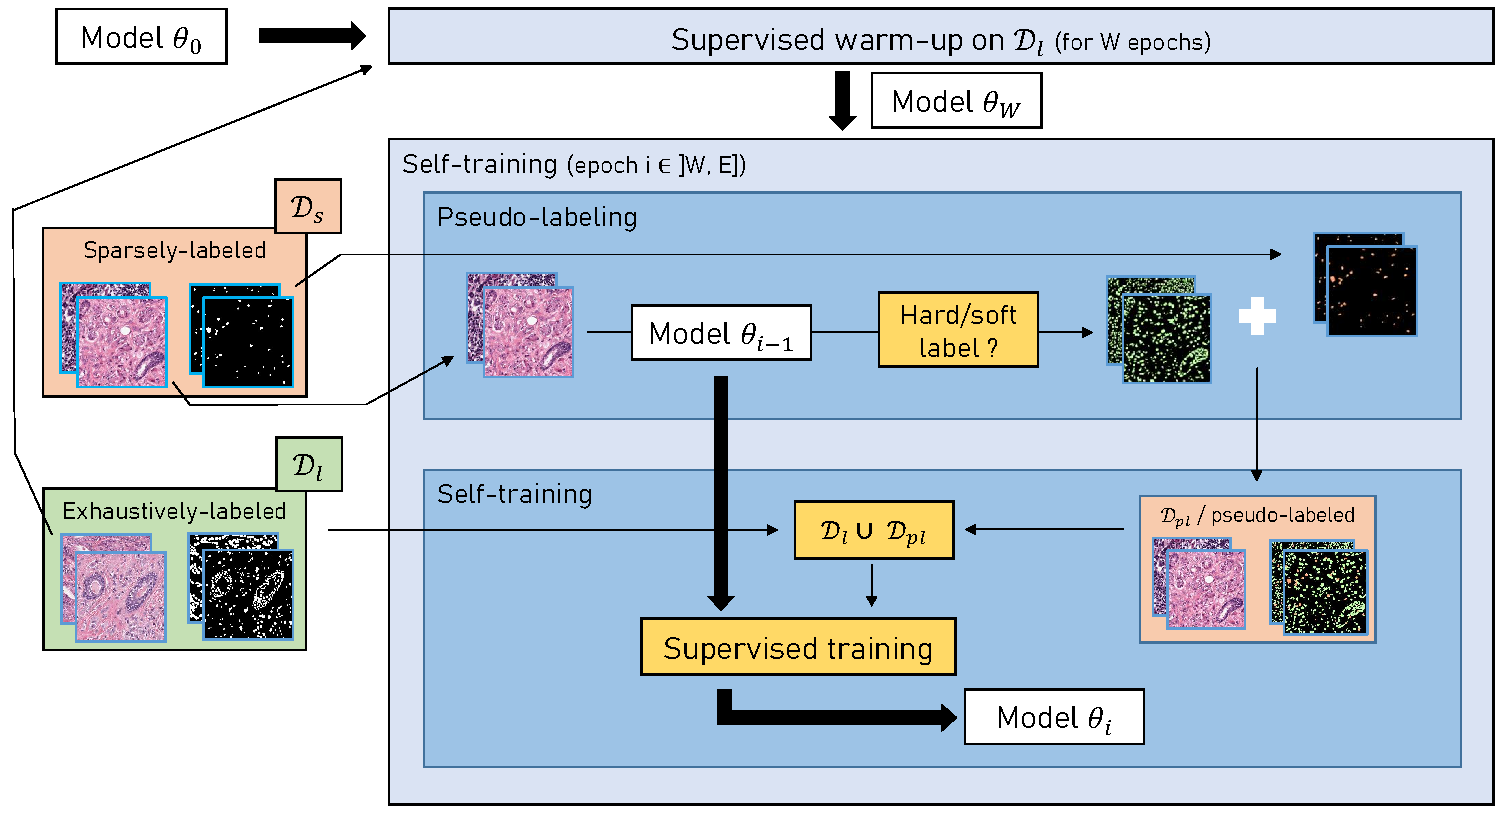
\includegraphics[width=\textwidth]{strain/method-diagram.pdf}
  \caption{Illustration of our self-training approach}
  \label{fig:strain:method_diagram}
\end{figure}

% Recent progresses in computing and artificial intelligence (AI) have created exciting opportunities the field of digital pathology. Nowadays, glass slides can be digitized into Whole-Slide Images (WSI) opening the way for AI-based analysis tools to relieve pathologists workload. Given the potentially dire consequences of misdiagnosis, these tools must be robust and reliable which can be challenging given the nature of the tasks and the different sources of variability affecting the WSI acquisition process. Machine learning techniques are considered some of the most promising tools to tackle these challenges but they often require a significant amount of training data to perform well. This is an issue in digital pathology which is considered to suffer from data scarcity \cite{tizhoosh2018artificial, litjens2017survey}: high-quality annotated pathology data are expensive and difficult to obtain. 

% This is the case in particular for structured output tasks such as image segmentation as exhaustive pixel-wise image labeling is a tedious task. When it comes to reducing the labeling cost, several approaches have been explored over the years: reducing the cost per annotation (\eg crowd-sourcing through citizen-science \cite{peplow2016citizen} or the intervention of junior pathologists and students \cite{amgad2021nucls}), reducing the time per annotation (\eg active learning and human-in-the-loop \cite{chai2020human}, dedicated annotation tools such as Cytomine \cite{maree2016collaborative}, interactive annotation \cite{berg2019}, or ai-assisted annotation \cite{amgad2021nucls, graham2021conic, aubreville2021mitosis}) or reducing the quantity of annotations needed in the first place (\eg use of external data trough transfer learning \cite{mormont2018comparison} or multi-task learning \cite{mormont2020multi})

%In this work, we are interested in the third category. More precisely, in order to reduce the required amount of annotated data, we study a labeling scheme where only a small subset of the available training data has to be exhaustively labeled whereas the rest can only be sparsely labeled, \TODO{or even left unlabeled}.  We evaluate how this labeling scheme can be exploited by learning methods to train efficient segmentation models. This learning problem belongs to semi-supervised learning and we use a self-training approach to tackle it.


\section{Methods}
\label{sec:strain:methods}

In the following section, we present our method, a self-training image segmentation algorithm. The self-training aspects and training implementation details are discussed separately in Sections \ref{ssec:strain:self_training} and \ref{ssec:strain:training_protocol} respectively.

We will denote by  $\mathcal{D} = \left(X, Y\right) \subset \mathcal{X} \times \mathcal{Y}$ a segmentation dataset, where $X$ and $Y$ respectively represent a set of input images and their corresponding binary segmentation masks. We will further consider a training dataset composed of two sets: $\mathcal{D}_l = \left(X_l, Y_l\right) \subset \mathcal{X} \times \mathcal{Y}$, the exhaustively labeled set, and $\mathcal{D}_s = \left(X_s, Y_s\right) \subset \mathcal{X} \times \mathcal{Y}$, the sparsely labeled set. In $\mathcal{D}_l$, the masks $Y_l$ are entirely determined, since the ground truth is known for all pixels (hence the exhaustiveness). In $\mathcal{D}_s$, ground truth is only partially known: given an image $\mathbf{x} \in X_s$, either a pixel $x_{ij}$ belongs to a structure of interest in which case the mask pixel $y_{ij} = 1$, or it is not labeled in which case $y_{ij} = 0$ and no assumption can be made a priori about the fact that the pixel belongs to a structure of interest or not. We will denote $n_l = |\mathcal{D}_l|$ and $n_s = |\mathcal{D}_s|$ the sizes of the sets. The total number of training images for a dataset will be denoted $n = n_l + n_s$.


\subsection{Self-training}
\label{ssec:strain:self_training}
 
Our self-training algorithm is described in Algorithm \ref{algo:strain:selftraining} (and depicted in Figure \ref{fig:strain:method_diagram}). It features a warm-up phase during which the model is classically trained on the set $\mathcal{D}_l$ (training implementation details are given in Section \ref{ssec:strain:training_protocol}). The number of warm-up epochs $W > 0$ is fixed so that the model is able to converge on the labeled data. The warmed-up model is used as starting point for the self-training phase. Each self-training round $e$ starts by pseudo-labeling $\mathcal{D}_s$ with the model $\theta_{e-1}$. For an image $\mathbf{x} \in X_s$, the pseudo-label assigned to pixel $x_{ij}$ is given by:
\begin{equation}
y^{({pl})}_{ij} = \begin{cases}
1,\,\text{if}\, y_{ij} = 1 \\
g(\hat{y}_{ij}),\,\text{otherwise}
\end{cases}
\label{eqn:strain:pseudolabeling}
\end{equation}
where $\hat{y}_{ij}$ is the sigmoid output of model $\theta_{e-1}$ for pixel $(i, j)$ given $\mathbf{x}$ as input and $g$ is a function for generating the pseudo-label from $\hat{y}_{ij}$ (see below). In other words, we preserve the expert ground truth as pseudo-labels when available and use the model predictions for unlabeled pixels (this is the \texttt{Combine} step from Algorithm \ref{algo:strain:selftraining}). With this strategy, entirely unlabeled images can also be included in $\mathcal{D}_s$. Our algorithm uses a single model (\ie teacher = student) which is not reset between self-training rounds. 

\begin{algorithm}[t]
  \SetAlgoLined
  \KwData{The exhaustively- and sparsely labeled sets $\mathcal{D}_l$ and $\mathcal{D}_s$, a segmentation model $\theta_0$, $W$ and $E$ respectively the number of warm up epochs and the total number of epochs.}
  \KwResult{A self-trained segmentation model $\theta_E$.}
  \SetKwFunction{Train}{Train}
  \SetKwFunction{Predict}{Predict}
  \SetKwFunction{Combine}{Combine}
  // \textit{Warm up}  \\
  \For{$e \leftarrow 1$ \KwTo $W$}{
    $\theta_e$ = \Train{$\theta_{e-1}, \mathcal{D}_l$}\;
  }
  \For{$e \leftarrow W+1$ \KwTo $E$}{
    // \textit{Pseudo labeling} \\
    $\hat{Y}_s =$ \Predict{$\theta_{e-1}, X_s$}\;  
    $Y_{pl} =$ \Combine{$\hat{Y}_s, Y_s$}\; 
    $\mathcal{D}_{pl} = \left(X_s, Y_{pl}\right)$\; 
    // \textit{Self-training} \\
    $\theta_e$ = \Train{$\theta_{e-1}, \mathcal{D}_l \cup \mathcal{D}_{pl}$}\;
  }
  \KwRet{$\theta_E$}
  \caption{Our self-training approach. The \texttt{Train} operation trains the given model on the provided dataset according to the protocol explained in Section \ref{ssec:strain:training_protocol}. The \texttt{Predict} operation produces segmentation masks for a set of input images using the model. The \texttt{Combine} operation combines ground truth masks and pseudo labels from the given sets as explained in Section \ref{ssec:strain:self_training}.}
  \label{algo:strain:selftraining}
\end{algorithm}

\subsubsection{Soft and hard pseudo-labels}
\label{sssec:strain:softandhardlabels}

We considered two different pseudo-labeling strategies, or two different $g$ functions (see Equation \ref{eqn:strain:pseudolabeling}). Initially, we decided to simply take $g$ to be the identity function $g(x) = x$ in which case the sigmoid output of the model was used as pseudo-label. This strategy is commonly called  ``\textit{soft}'' labeling. During the next self-training round, this soft label will be compared to the network prediction which can be seen as a form of consistency constraint similar to those in \cite{laine2016temporal,tarvainen2017mean,sohn2020fixmatch}. However, early experiments have shown that this approach causes training instabilities. Therefore, we investigated a second strategy where the sigmoid output is binarized using a threshold $T_e \in [0, 1]$:
\begin{equation}
g(x) = \begin{cases}
1,\,\text{if}\, x > T_e\\
0,\,\text{otherwise}
\end{cases}
\end{equation}   
where $e$ is a self-training round. We call this strategy ``\textit{hard}'' labeling as pseudo-labels are either 0 or 1. In addition to ensuring some sort of consistency between the pseudo-labels and the predictions, as in the ``\textit{soft}'' approach, this thresholding also encourages the model to produce confident predictions (closer to 0 or 1). Because we want to avoid $T_e$ to be an additional hyperparameter to tune, we propose an auto-calibration strategy based on the Dice score: 
\begin{equation}
  Dice_T(\mathbf{y},\hat{\mathbf{y}}) = \dfrac{2 \times \sum_{i,j} \left[\mathbb{1}_{\hat{y}_{ij} \geq T} \times y_{ij}\right]}{\sum_{i,j} \mathbb{1}_{\hat{y}_{ij} \geq T} + \sum_{i,j} y_{ij}}
  \label{eqn:strain:dice}
\end{equation}
where $T$ is the threshold applied to the model output to generate a binary prediction. The auto-calibration procedure selects $T_e$ such that the Dice score in (\ref{eqn:strain:dice}) is maximized for the images from an exhaustively labeled set  $\mathcal{D}_{a}$:
\begin{equation}
T_e = \arg \underset{T}{\max} \sum_{(\mathbf{x}, \mathbf{y}) \in \mathcal{D}_a} \text{Dice}_T\left(\mathbf{y},h( \mathbf{x}; \theta_{e})\right).
\label{eqn:strain:thresholdopt}
\end{equation}
The ideal choice for $\mathcal{D}_{a}$ would be to use an external validation set but, in extreme data scarcity conditions, extracting such a validation set would penalize the performance of the algorithm by removing a significant amount of training data. Therefore, in this context, we consider using the training subset $\mathcal{D}_l$ as $\mathcal{D}_a$.
This approach has the advantage of not requiring additional training data but also induces a risk of overfitting which might hurt generalization performance. We hope that the overfitting problem would be compensated by the improvement brought by hard labeling. 
A performance comparison of these two pseudo-labeling strategies is given in Section \ref{ssec:strain:res:hardvssoft} and motivates the use of the second strategy.

\subsection{Training}
\label{ssec:strain:training_protocol}

In this section, we will provide more information about the \texttt{Train} procedure from Algorithm \ref{algo:strain:selftraining} which trains a model $\theta$ with a dataset $\mathcal{D}$.
We use U-Net \cite{ronneberger2015unet} as a segmentation architecture. We set the initial number of feature maps to 8 instead of 64 in the original article, with the rest of the network scaled accordingly. The main goal of this reduction of model capacity is to limit overfitting given the highly scarce data conditions explored in this work, but it would be worth exploring more complex architectures as future work.

%This reduction of model capacity was chosen arbitrarily and motivated by the fact that we study mostly highly scarce data conditions in this work. Therefore, using a lower capacity model seemed relevant as less training data is available \NOTE{tjrs pas tout a fait satisfait de la manière dont ça sonne}. 

The number of rounds $W$ and $E$ and the number of training iteration per round are chosen independently per dataset (see Supplementary Section \ref{app:strain:sec:expfixednl}). Every training iteration, we build a minibatch by sampling $B=8$ images uniformly at random with replacement from $\mathcal{D}_l \cup \mathcal{D}_{pl}$ and by extracting one randomly located 512x512 patch and its corresponding mask from each of these images. The batch size was selected based on hardware memory constraints. We apply random data augmentation following best practices for machine learning in general and for self-training in particular \cite{xie2020self,sohn2020fixmatch}. We apply horizontal and vertical flips, color perturbation in the HED space \cite{tellez2018whole} (bias and coefficient factors up to 2.5\%), Gaussian noise (standard deviation up to 10\%) and Gaussian blur (standard deviation up to 5\%). 

As a training loss, we average the per-pixel binary cross-entropy $\ell$ over all pixels of the batch, as defined in:
\begin{align}
\ell(\hat{y}; y) = y \log \hat{y} + (1 - y) \log (1 - \hat{y}) \label{eqn:strain:perpixel_crossentropy} \\
\mathcal{L} = - \frac{1}{B} \sum_{b=1}^B \frac{1}{|\mathbf{y}_b|}\sum_{i}\sum_{j} w_{ij, b} \ell(\hat{y}_{ij, b}; y_{ij,b }) 
\label{eqn:strain:overallloss}
\end{align}

We multiply the per-pixel loss by a weight $w_{ij, b}$ for pixel $(i, j)$ of the $b^{th}$ image of the batch in order to tune the contribution of this pixel to the loss (see Section \ref{sssec:strain:weights}).
We use Adam \cite{kingma2014adam} as an optimizer with initial learning rate $\gamma= 0.001$ and default hyperparameters ($\beta_1 = 0.9$, $\beta_2 = 0.999$, no weight decay).


\subsubsection{Weighting schemes}
\label{sssec:strain:weights}

Different strategies are evaluated for generating the per-pixel weight $w_{ij,b}$ in Equation \ref{eqn:strain:overallloss}. For the sake of simplicity, we will drop the batch identifier $b$ in the subsequent equations and denote this weight by $w_{ij}$. We introduced this weight term to have the possibility to tune the contribution of pseudo-labeled pixels when computing the loss. It is important to note that this weight only applies to pseudo-labeled pixels and, therefore, the ground truth pixels will always be attributed a weight of $w_{ij} = 1$. It is also important to note that the weight is inserted as a constant in our loss and the weight function is not differentiated during back-propagation. 

We study five different weighting strategies each producing an intermediate weight $w^{\xi}_{ij}$ where $\xi$ is the strategy identifier. Because we want to avoid the amplitude of the loss and gradients to be impacted by the weighting strategy, we normalize it to obtain the final weight $w_{ij} = w^{\xi}_{ij}/\overline{w}^{\xi},$
%\begin{equation}
%$w_{ij} = \dfrac{w^{\xi}_{ij}}{\overline{w}^{\xi}},$
%\end{equation}
where $\overline{w}^{\xi}$ is the average weight over all pixels of a patch. Our weighting strategies are as follows:

\paragraph{Constant.} This strategy consists in setting $w^{\text{cst}}_{ij} = C$ where $C \in \mathbb{R}^+$ is an hyperparameter. Because $w_{ij} = 1$ for ground truth pixels, this allows to manually balance the relative contributions of ground truth and pseudo-labeled pixels. The special case $C = 1$ assigns the same weight to ground truth and pseudo-labels and therefore corresponds to removing $w_{ij,b}$ from Equation \ref{eqn:strain:overallloss}.

\paragraph{Balance} This strategy automatically assigns a value to the $C$ hyperparameter presented in the ``constant'' strategy. As a basis for this value, we use the ratio $g$ of ground truth pixels in $\mathcal{D}_l \cup \mathcal{D}_s$. The final weight is given by: 
\begin{equation}
w^{\text{bal}}_{ij} = \frac{g}{1 - g}.
\label{eqn:strain:balancegt}
\end{equation}
This choice is motivated by the belief that our algorithm will provide more reliable pseudo-labels in a low data scarcity regime ($g \nearrow $) in which case it makes sense to tune up the contributions of those pseudo-labels to the loss. In the opposite situation of extreme data scarcity ($g \searrow $), we expect the algorithm to produce less reliable pseudo-labels. 

\paragraph{Entropy} \label{par:strain:entropyweight} Unlike the previous, this strategy is not concerned with balancing the contributions but instead penalizes pseudo-labels for which the model was uncertain. It considers the prediction $\hat{y}_{ij}$ as a probability and tune the contribution down using the Shannon entropy. The use of entropy is motivated by its use in several self-training methods \cite{grandvalet2004semi,lee2013pseudo}. First, an intermediate weight $\omega_{ij}$ is computed as: 
\begin{equation}
\omega_{ij} = 1 + \hat{y}_{ij} \log_2(\hat{y}_{ij}) + (1 - \hat{y}_{ij}) \log_2(1 - \hat{y}_{ij}).
\label{eqn:strain:entropyweight}
\end{equation}
Early experiments have shown that directly using $\omega_{ij}$ as a weight resulted in unstable training. Indeed, during early self-training rounds, the model typically produces $\hat{y}_{ij} \sim 0.5$ which results in $\omega_{ij} \sim 0$ for most pixels in a patch, leaving only foreground ground truth pixels to be evaluated in the loss. In order to avoid this behavior, we introduce a new hyperparameter $w_{min} \in \left]0, 1\right]$ which allows rescaling linearly the weights $\omega_{ij}$ to $w^{ent}_{ij} \in [w_{min},1]$ as defined in:
\begin{equation}
w^{ent}_{ij} = \left(1 - w_{\text{min}}\right) \omega_{ij} + w_{\text{min}}.
\label{eqn:strain:wminrescale}
\end{equation}

\paragraph{Consistency.} Self-training algorithms often enforce consistency between the teacher and student models predictions. Inspired from this, we exploit another form of consistency for this strategy. In structured output tasks like segmentation, there is a correlation between predictions that are spatially close, as, for most pixels, it is unlikely that the true label should differ between a pixel and its neighbors. Therefore, we use the pseudo-label consistency between a pixel and its neighbors as a proxy to evaluate reliability of this pseudo-label: %The weight is given by
\begin{equation}
w^{\text{cty}}_{ij} = 1 - \dfrac{\sum_{k=-\eta}^{\eta} \sum_{l=-\eta}^{\eta} (\hat{y}_{ij}- \hat{y}_{(i+k)(j+l)})^2}{\eta^2 - 1}
\end{equation}
where $\eta$ is the size of the neighborhood and an hyperparameter of the method. We consider a square neighborhood around the central pixel and ignore pixels outside of the image at the image borders. We have arbitrarly chosen $\eta = 2$ as default value for all our experiments involving the ``\textit{consistency}'' weighting strategy. This means that each pixel (except at the image borders) is compared to 24 neighboring pixels when computing consistency. 

\paragraph{Merged.} This strategy assigns a high weight to pixels for which the model is both certain and consistent (spatially). It achieves this by multiplying together the consistency weight $w^{\text{cty}}_{ij}$ and the entropy raw weight $\omega_{ij}$. Because $\omega_{ij}$ suffers from the issue described earlier, we apply the same re-scaling operation after multiplication:
\begin{equation}
w^{\text{mgd}}_{ij} = (1 - w_{min}) \left(w^{\text{cty}}_{ij} \times \omega_{ij}\right) + w_{min}.
\end{equation}

\section{Data}
\label{sec:strain:data}

In this section, we describe the datasets we use to evaluate our method. It includes three public exhaustively labeled segmentation datasets: \acrshort{monuseg} \cite{kumar2019multi}, \acrshort{glas} \cite{sirinukunwattana2017gland} and \acrshort{segpc} \cite{gupta2021segpc}. The datasets are described in Table \ref{tab:strain:datasets_statistics} and illustrated in Figure \ref{fig:strain:datasets_samples}. \acrshort{monuseg} contains images of tissues coming from different organs, patients and hospitals where epithelial and stromal nuclei are annotated. Given the variety of sources, the images exhibit significant variations of staining and morphology. The density of annotations is also quite high compared to the other datasets. \acrshort{glas} features images containing both benign tissues and malignant tissues with colonic carcinomas. The gland annotations vary greatly in shape and size. Originally, \acrshort{segpc} contains 3 classes: background, cytoplasm and nucleus. In this work, we merge the two latter classes as we focus on binary segmentation. One of the challenges of this dataset is the presence of non-plasma cells which should be ignored by the algorithm although they are very similar to plasma cells. Moreover, artefacts are present on the images (\eg cracked scanner glass in foreground, scale reference or magnification written on the image).

\begin{table}
  \centering
  \begin{tabular}{|c|cc|cc|}
    \hline
    \multirow{2}{*}{Dataset} & \multicolumn{2}{c|}{Training set} & \multicolumn{2}{c|}{Test set}\\
    & Images & Annots    & Images & Annots  \\
    \hline
    \acrshort{monuseg} & 30 & 17362 & 14 & 11484\\
    \acrshort{glas} & 85 & 763 & 80 & 781 \\
    \acrshort{segpc} & 298 & 1643 & 300 & 900 \\
    \hline
  \end{tabular}
  \caption{Summary statistics for the four datasets used in this work. An image is a region of interest extracted from a whole-slide image.}
  \label{tab:strain:datasets_statistics}
\end{table}


\begin{figure}
  \centering
  \begin{subfigure}{0.48\textwidth}
    \centering
    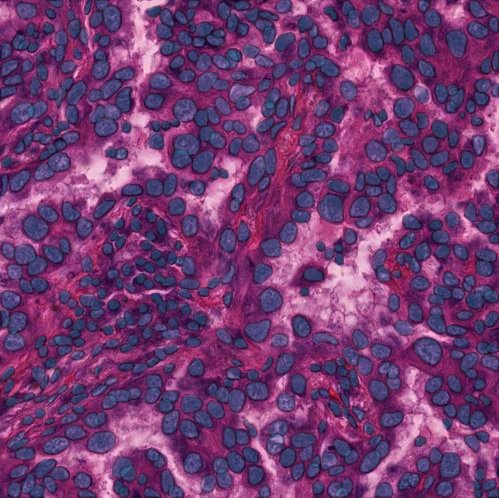
\includegraphics[width=\textwidth]{strain/monuseg_sample1.png}
    \caption{\acrshort{monuseg}}
    \label{sfig:strain:monuseg_sample1}
  \end{subfigure}
  \begin{subfigure}{0.48\textwidth}
    \centering
    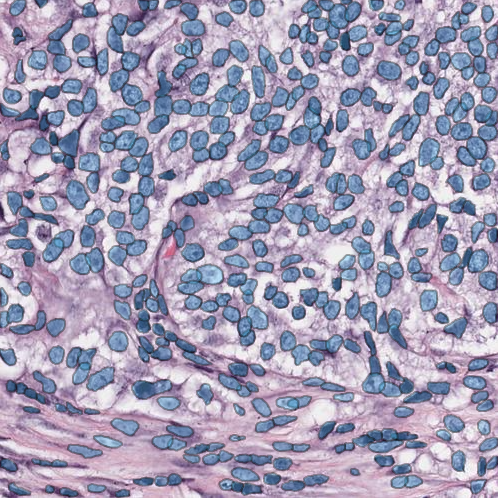
\includegraphics[width=\textwidth]{strain/monuseg_sample2.png}
    \caption{\acrshort{monuseg}}
    \label{sfig:strain:monuseg_sample2}
  \end{subfigure} \\

  \begin{subfigure}{0.48\textwidth}
    \centering
    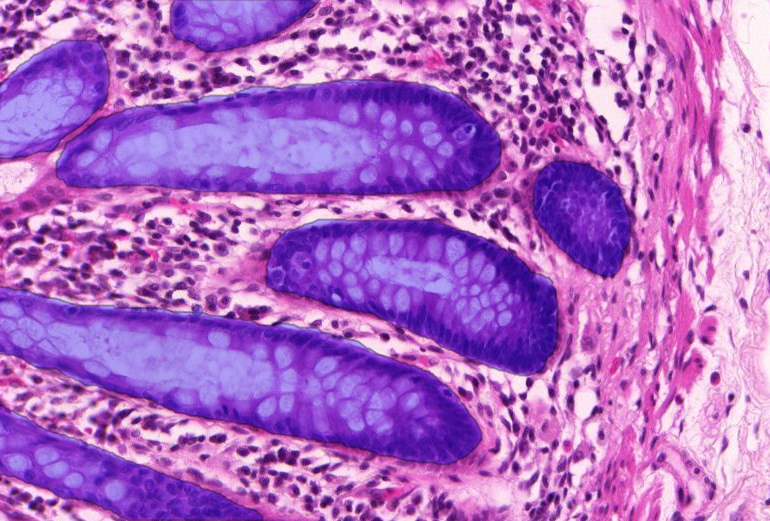
\includegraphics[width=\textwidth]{strain/glas_sample1.png}
    \caption{\acrshort{glas}}
    \label{sfig:strain:glas_sample1}
  \end{subfigure}
  \begin{subfigure}{0.48\textwidth}
    \centering
    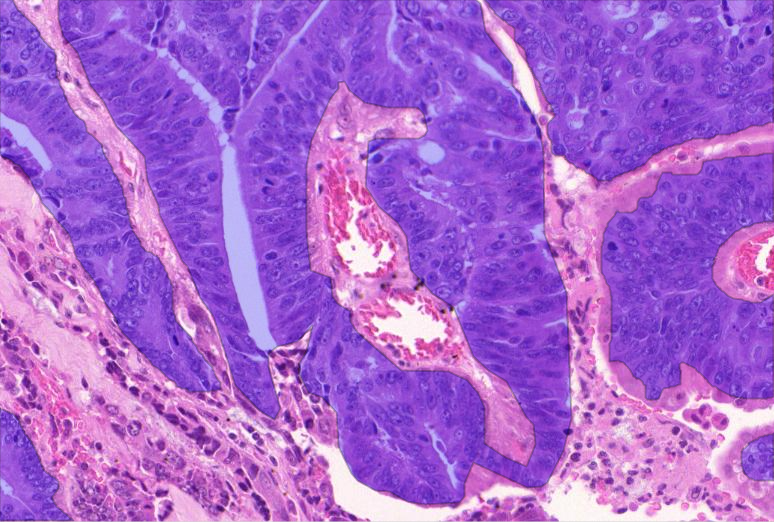
\includegraphics[width=\textwidth]{strain/glas_sample2.png}
    \caption{\acrshort{glas}}
    \label{sfig:strain:glas_sample2}
  \end{subfigure} \\

  \begin{subfigure}{0.48\textwidth}
    \centering
    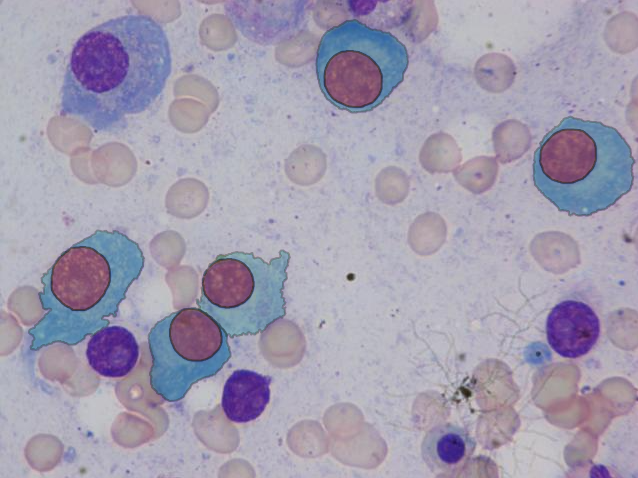
\includegraphics[width=\textwidth]{strain/segpc_sample1.png}
    \caption{\acrshort{segpc}}
    \label{sfig:strain:segpc_sample1}
  \end{subfigure}
  \begin{subfigure}{0.48\textwidth}
    \centering
    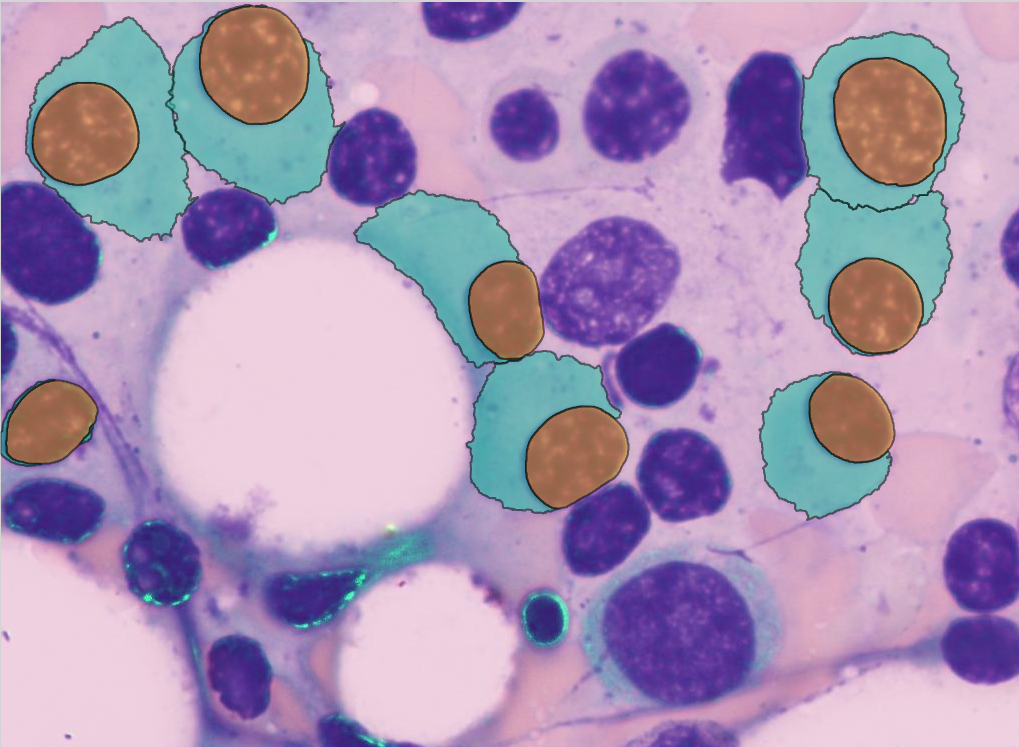
\includegraphics[width=\textwidth]{strain/segpc_sample2.png}
    \caption{\acrshort{segpc}}
    \label{sfig:strain:segpc_sample2}
  \end{subfigure} 
  
  \caption{Samples from \acrshort{monuseg}, \acrshort{glas} and \acrshort{segpc} used in this work.}
  \label{fig:strain:datasets_samples}
\end{figure}

\subsection{Thyroid \acrshort{fnab}}
\label{ssec:strain:thyroidfnab}

In addition to the three public datasets, we use a dataset that actually motivated the development of our method, a sparsely labeled dataset for thyroid nodule malignancy assessment. Pathologists\footnote{ULB Erasme hospital, Belgium, team of Pr. Isabelle Salmon.} sparsely annotated nuclear features (see Figure \ref{fig:strain:cells_examples}) and architectural patterns (see Figure \ref{fig:strain:patterns_examples}) with polygon annotations in 85 whole-slide images using Cytomine \cite{maree2016collaborative}. Each polygon was associated with a term from the ontology given in Supplementary Section \ref{app:strain:sec:thyroidontology}. The training set consists of 4742 crops, one for each polygon annotation. The test set is a set of 45 regions of interest (2000x2000 pixels each) with annotations highlighting structures of interest (binary annotations, background \vs nuclei features and architectural cell patterns) made by a computer science student.

Given how the labeling process was carried out, we hypothesize that crops of architectural patterns are less likely to contain unlabeled cells than crops of nuclear features. Indeed, the former usually consist in large polygons delineating areas containing cell aggregates. Nuclear features, unlike architectural patterns, were usually labeled more sparsely and it is frequent to find annotations of a single cell within an unlabeled cell aggregate. From these observations, we have decided to assign the architectural patterns to $\mathcal{D}_l$ and nuclear features to $\mathcal{D}_s$.


\begin{figure}
    \centering
    \begin{subfigure}{.48\textwidth}
      \centering
      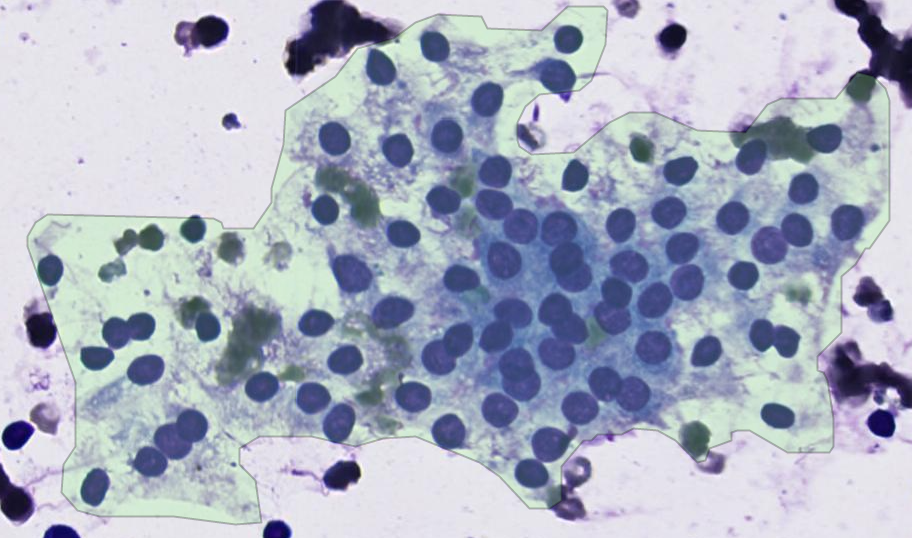
\includegraphics[width=\textwidth]{strain/patterns1.png}
      \caption{}
      \label{sfig:strain:pattern1}
    \end{subfigure}
    \begin{subfigure}{.48\textwidth}
      \centering
      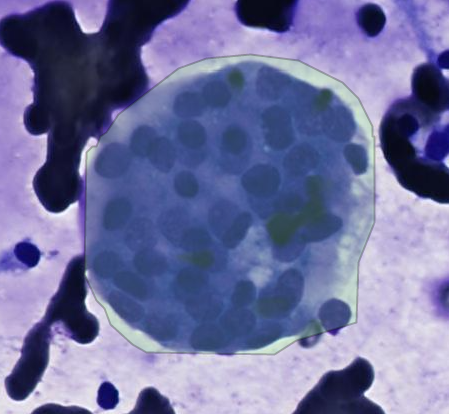
\includegraphics[width=\textwidth]{strain/patterns2.png}
      \caption{}
      \label{sfig:strain:pattern2}
    \end{subfigure} \\
    \begin{subfigure}{.48\textwidth}
      \centering
      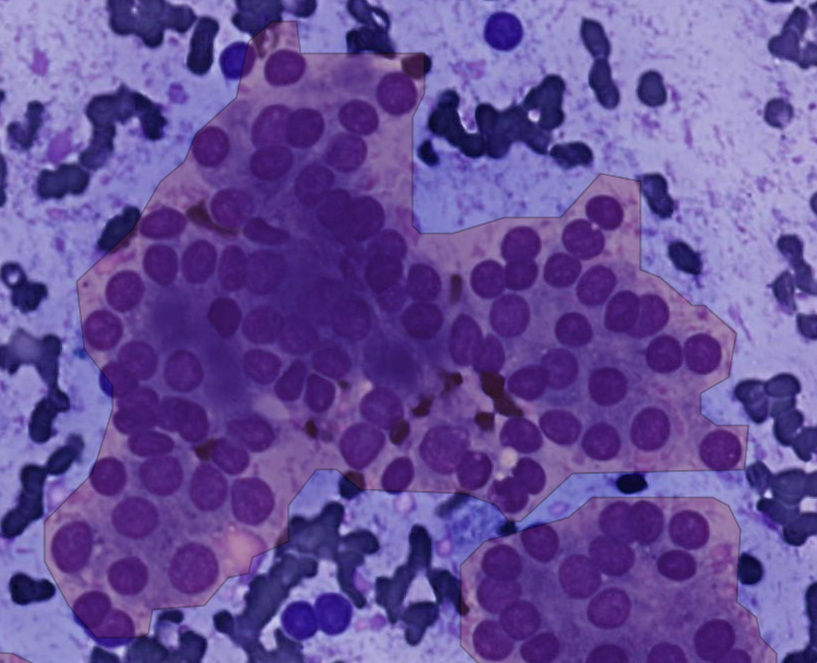
\includegraphics[width=\textwidth]{strain/patterns3.png}
      \caption{}
      \label{sfig:strain:pattern3}
    \end{subfigure}
    \begin{subfigure}{.48\textwidth}
      \centering
      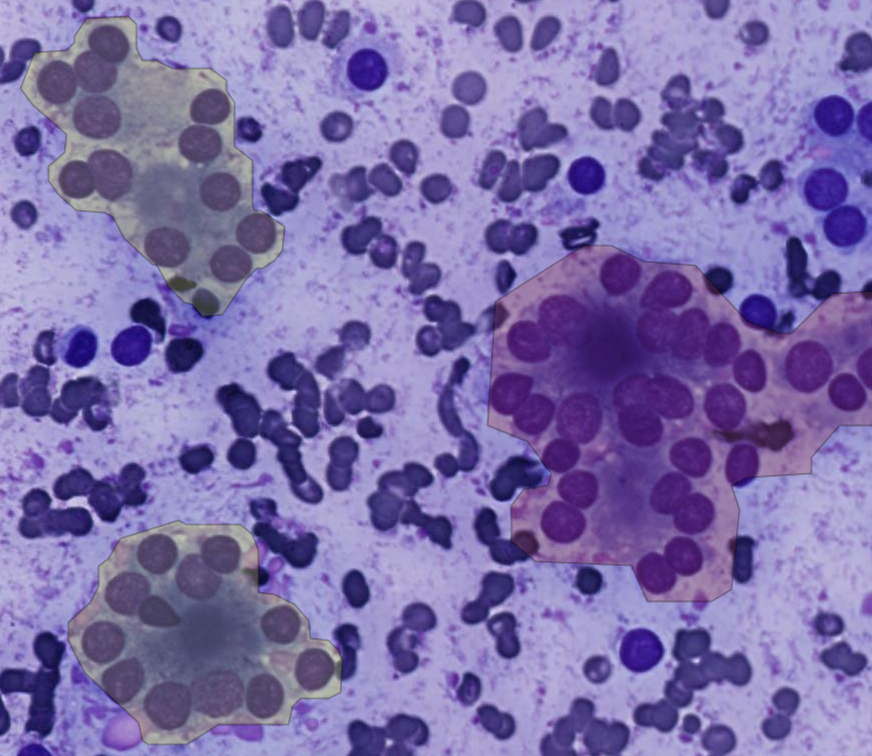
\includegraphics[width=\textwidth]{strain/patterns4.png}
      \caption{}
      \label{sfig:strain:pattern4}
    \end{subfigure}
    \caption{Examples of architectural patterns annotations made by pathologists for Thyroid \acrshort{fnab}.}
    \label{fig:strain:patterns_examples}
\end{figure}


\begin{figure}
    \centering
    \begin{subfigure}{.235\textwidth}
      \centering
      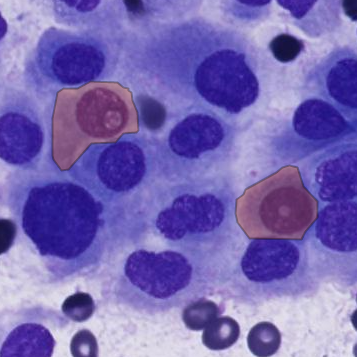
\includegraphics[width=\textwidth]{strain/cells1.png}
      \caption{}
      \label{sfig:strain:cell1}
    \end{subfigure}
    \begin{subfigure}{.235\textwidth}
      \centering
      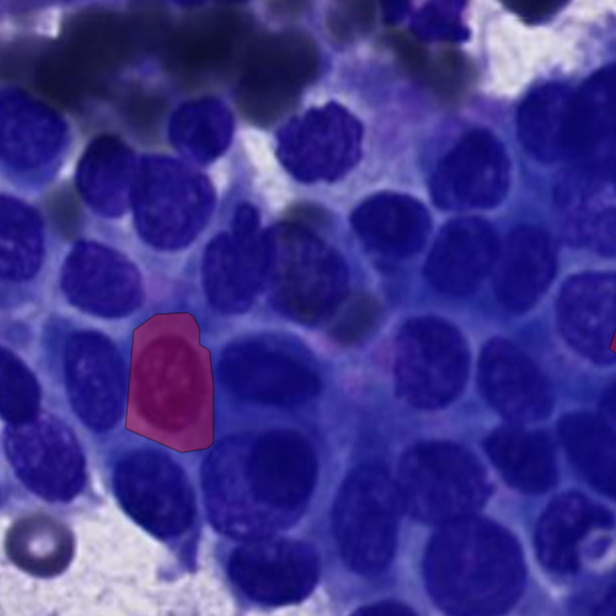
\includegraphics[width=\textwidth]{strain/cells2.png}
      \caption{}
      \label{sfig:strain:cell2}
    \end{subfigure}
    \begin{subfigure}{.235\textwidth}
      \centering
      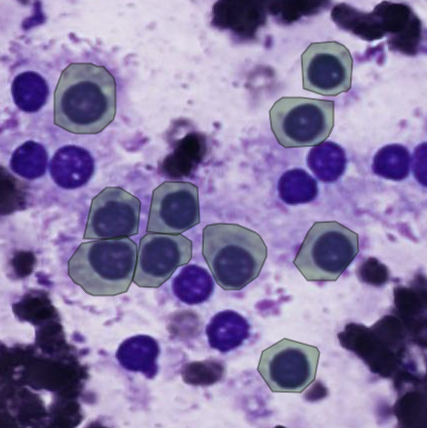
\includegraphics[width=\textwidth]{strain/cells3.png}
      \caption{}
      \label{sfig:strain:cell3}
    \end{subfigure}
    \begin{subfigure}{.235\textwidth}
      \centering
      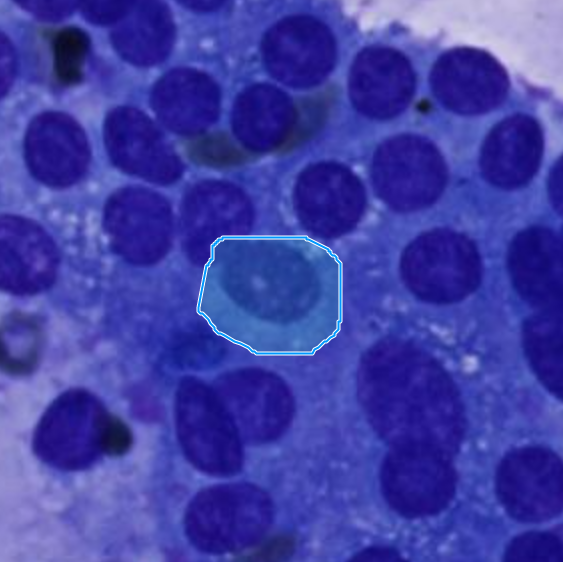
\includegraphics[width=\textwidth]{strain/cells4.png}
      \caption{}
      \label{sfig:strain:cell4}
    \end{subfigure}
    \caption{Examples of nuclear features annotations made by pathologists for Thyroid \acrshort{fnab}.}
    \label{fig:strain:cells_examples}
\end{figure}


\section{Experimental setup}
\label{sec:strain:experiments}

In this section, we present context information for our experiments: what are our baselines, how we have simulated sparse datasets from the public datasets and what evaluation protocol we have applied.

\subsection{Transforming the datasets}

In order to fit the sparsely labeled settings described in Section \ref{sec:strain:methods}, we generate new datasets from \acrshort{segpc}, \acrshort{glas} and \acrshort{monuseg}. This generation is controlled by two parameters: $n_l$ and $\rho$. The former is the number of images to keep in the exhaustively labeled set $\mathcal{D}_l$. These images are chosen at random without replacement in the original training set. The latter parameter $\rho$ is the percentage of annotations to remove from the images to make the remaining images sparsely labeled.

For \acrshort{monuseg}, we remove $\rho \%$ of the instances in each image selected for the sparse set. For \acrshort{segpc} and \acrshort{glas}, because the number of instances per image is small (up to two or three dozen), we remove $\rho \%$ of the instances from the complete list of instances. As a result, some sparse training images from these  datasets can be completely void of ground truth. However, this is not a problem as our pseudo-labeling process is designed to support such images. 

\subsection{Baselines}
\label{ssec:strain:baselines}

We compare our self-training approach to three baselines. The first one, referred to as ``\textit{upper}'', consists in using the full dataset, without removing any ground truth (\ie $|\mathcal{D}_l| = n$ and $|\mathcal{D}_s| = 0$). Since it has access to all the annotations, this baseline is expected to represent an upper bound for all other strategies. 

The second baseline consists in using the sparsely-annotated set $\mathcal{D}_s$ as if it was exhaustively annotated ($\mathcal{D}_{train} = \mathcal{D}_l \cup \mathcal{D}_s$). This strategy makes sense especially for moderately sparse datasets. Indeed, convolutional layers (as in U-Net) are able to cope with a bit of label noise given that gradients are averaged over feature maps to update the model parameters. Therefore, a bit of noise in certain parts of the images can be compensated by the feedback of ground truth labels in other locations. This baseline will be referred to as ``$\mathcal{D}_l \cup \mathcal{D}_s$''.

The third and last baseline, referred to as ``\textit{$\mathcal{D}_l$ only}'', consists in not using at all the sparsely-annotated images during the training process (\ie $\mathcal{D}_{train} = \mathcal{D}_l$).

Our self-training approach is of practical interest if it outperforms the two latter baselines. Moreover, the closer to the ``\textit{upper}'' baseline the better.

\subsection{Evaluation}
\label{ssec:strain:evaluation}

We have built an evaluation protocol in order to ensure a fair comparison between the different strategies and the baselines. Ultimately, all approaches produce a segmentation model $\theta$ that will be the one evaluated. As an evaluation metric, we use the Dice score introduced in Equation \ref{eqn:strain:dice} which requires a threshold $T$ to turn the probability map produced by the model into a binary segmentation. To assess the performance of a model independently of the thresholding strategy, we pick $T$ so that the Dice score is maximized on the test set. In other words, in order to determine the threshold, we apply the optimization procedure described in Equation \ref{eqn:strain:thresholdopt} where $\mathcal{D}_a$ is the test set $\mathcal{D}_{\text{test}}$. The Dice score resulting from this optimization will be referred to as ``$\text{Dice}^*$''. Obviously, in a context of extreme data scarcity, it will not be possible to tune the threshold this way because of the lack of a sufficiently large validation or test set. We will leave the design of fully automatic strategies to tune such threshold as future work but we believe that visually tuning such threshold on new images would be feasible in interactive applications where the segmentation models would be mostly used to assist the labeling of new images.

Every experiment and hyperparameters combination we evaluate is run with ten random seeds to evaluate the variability. The seed affects the dataset sparsity ($n_l$ and $\rho$), model initialization, mini-batch sampling and data augmentation. We report Dice average and standard deviation over these random seeds.  

% \paragraph{Manual threshold tuning} As previously explained, we tune the threshold on $\mathcal{D}_l$ for most experiments which implies a risk of overfitting. Therefore, we wanted to try another strategy. In practice, one could imaging a setup where a human would run the algorithm and generate $\theta$ then set $T$ by tuning it manually on a few test images. This protocol raises questions related to bias (human-related) and small sample size but depending on the final application (\eg AI-assisted annotation), they might not really be an issue. This protocol would also alleviate the issue of training set overfitting. 

% Therefore, we have re-evaluated the models generated during our experiments using a similar protocol similar to leave-one-out cross-validation. Given a run of our algorithm, we have extracted the final model $\theta$ and the associated random seed $r$. The seed was used to randomly extract $K$ images from the related test set $\mathcal{D}_t$ which were used to tune the threshold $T$. For the sake of simplicity, instead of using a human, we have applied the same threshold optimization procedure based on the Dice score as presented in Section \ref{sssec:strain:softandhardlabels} for hard labels. The threshold was then used to evaluate the model on the remaining $|\mathcal{D}_t| - K$ images. We have repeated this procedure for all seeds and then average the results. This process is similar to a non-exhaustive $K$-fold cross validation. 

\section{Experiments and results}
\label{sec:strain:results}

\subsection{Hard \vs soft pseudo-labeling}
\label{ssec:strain:res:hardvssoft}

\TODO{discuter de cette section, revoir section méthode "hard vs soft" pour qu'elle soit cohérente} 

In this section, we explore how the two choices of pseudo-label generation presented in Section \ref{sssec:strain:softandhardlabels} impact the performance of self-training. In order to answer this question, we have run our self-training approach with different hyperparameter settings either with hard or soft pseudo-labels. We have performed 10 runs per hyperparameter combination and considered 24 combinations for \acrshort{segpc}, 20 for \acrshort{monuseg} and 22 for \acrshort{glas} (see Supplementary Section \ref{app:strain:sec:hardvssoft} for a detailed list of hyperparameters combinations). This experiment was carried out during the exploratory phase of the work where we studied a significantly scarce regime with $\rho = 90\%$ for all datasets and $n_l$ set to $2$ for \acrshort{monuseg}, $30$ for \acrshort{segpc} and $8$ for \acrshort{glas} (\ie between $90\%$ and $95\%$ of sparsely labeled images with $90\%$ of missing annotations).

The resulting performance are reported in Figure \ref{fig:strain:hard_vs_soft}. We observe that, for all datasets except \acrshort{glas}, the range of performance obtained with soft pseudo-labels fits within the range of performance of hard pseudo-labels. This indicates that soft labels yield more stable performance and are less impacted by the choice of a weighting strategy and its hyperparameters. This also seems to indicate that when appropriately selecting the hyperparameters, hard pseudo-labels are able to produce better performance. However, it also means that a bad choice of self-training hyperparameters when using hard labels would have a more significative negative on the performance . For \acrshort{glas}, the performance obtained using soft labels are inferior to those of hard labels. 

As a disclaimer, this analysis holds for the studied scarcity regime as the impact of hard and soft pseudo-labels could change in different conditions which we have not evaluated due to time and computational resources constraints. 

\begin{figure}
  \centering
  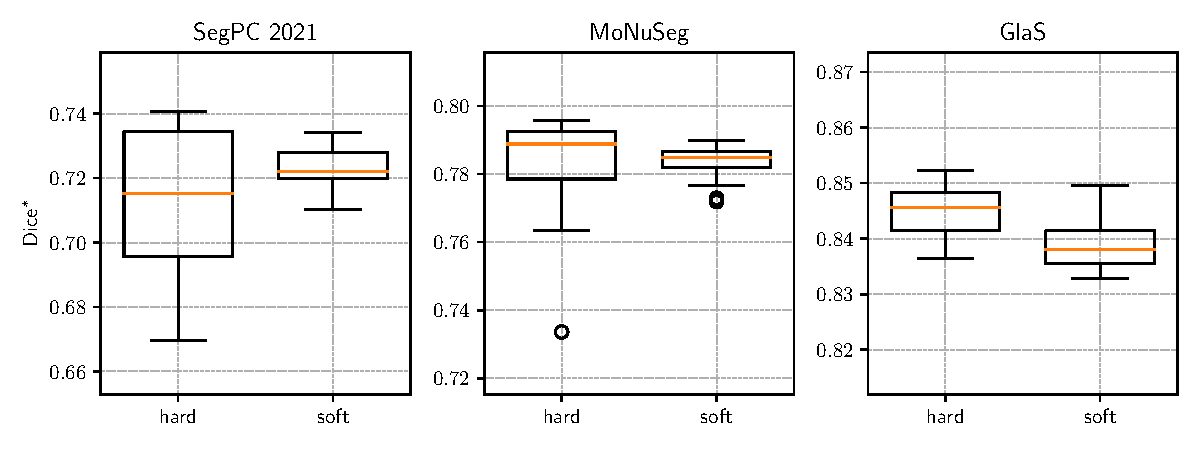
\includegraphics[width=\textwidth]{strain/plot_hard_vs_soft_test_pxl_self_hard_dice.pdf}
  \caption{Comparing performance between using self-training with hard and soft labels.}
  \label{fig:strain:hard_vs_soft}
\end{figure}

\subsection{Self-training performance at fixed $n_l$}
\label{ssec:strain:fixednl}

In order to study how our self-training approach performs under different data scarcity conditions, we have generated several versions of our datasets by varying $\rho$ with $n_l$ fixed and have run the baselines and different hyperparameters combinations on the generated datasets. As discussed in Sections \ref{ssec:strain:self_training} and , we have used hard labels exclusively. The detailed hyperparameter combinations used in this section are provided in Supplementary Section \ref{app:strain:sec:expfixednl}.

Results are shown for all three datasets in Figure \ref{fig:strain:rho_exp}. In general, self-training is always able to outperform significantly the ``\textit{$\mathcal{D}_l$ only}'' and ``$\mathcal{D}_l \cup \mathcal{D}_s$'' baselines with a significantly reduced amount of sparse annotations (the exact value is dataset dependant, see below). Regarding the baselines, ``\textit{upper}''  outperforms the two others. Moreover, using sparsely labeled images as if they were exhaustively labeled (\ie $\mathcal{D}_l \cup \mathcal{D}_s$) appears not to be a good idea as it is outperformed by all self-training approaches and baselines in almost all scarcity conditions. The performance of this baseline increases as one adds more sparse annotations however and is able to catch up with the ``\textit{$\mathcal{D}_l$ only}'' baseline in the lowest scarcity conditions validating the hypothesis presented in Section \ref{ssec:strain:baselines}. 

\begin{figure}[th]
  \centering
    \begin{subfigure}{\textwidth}
    \centering
    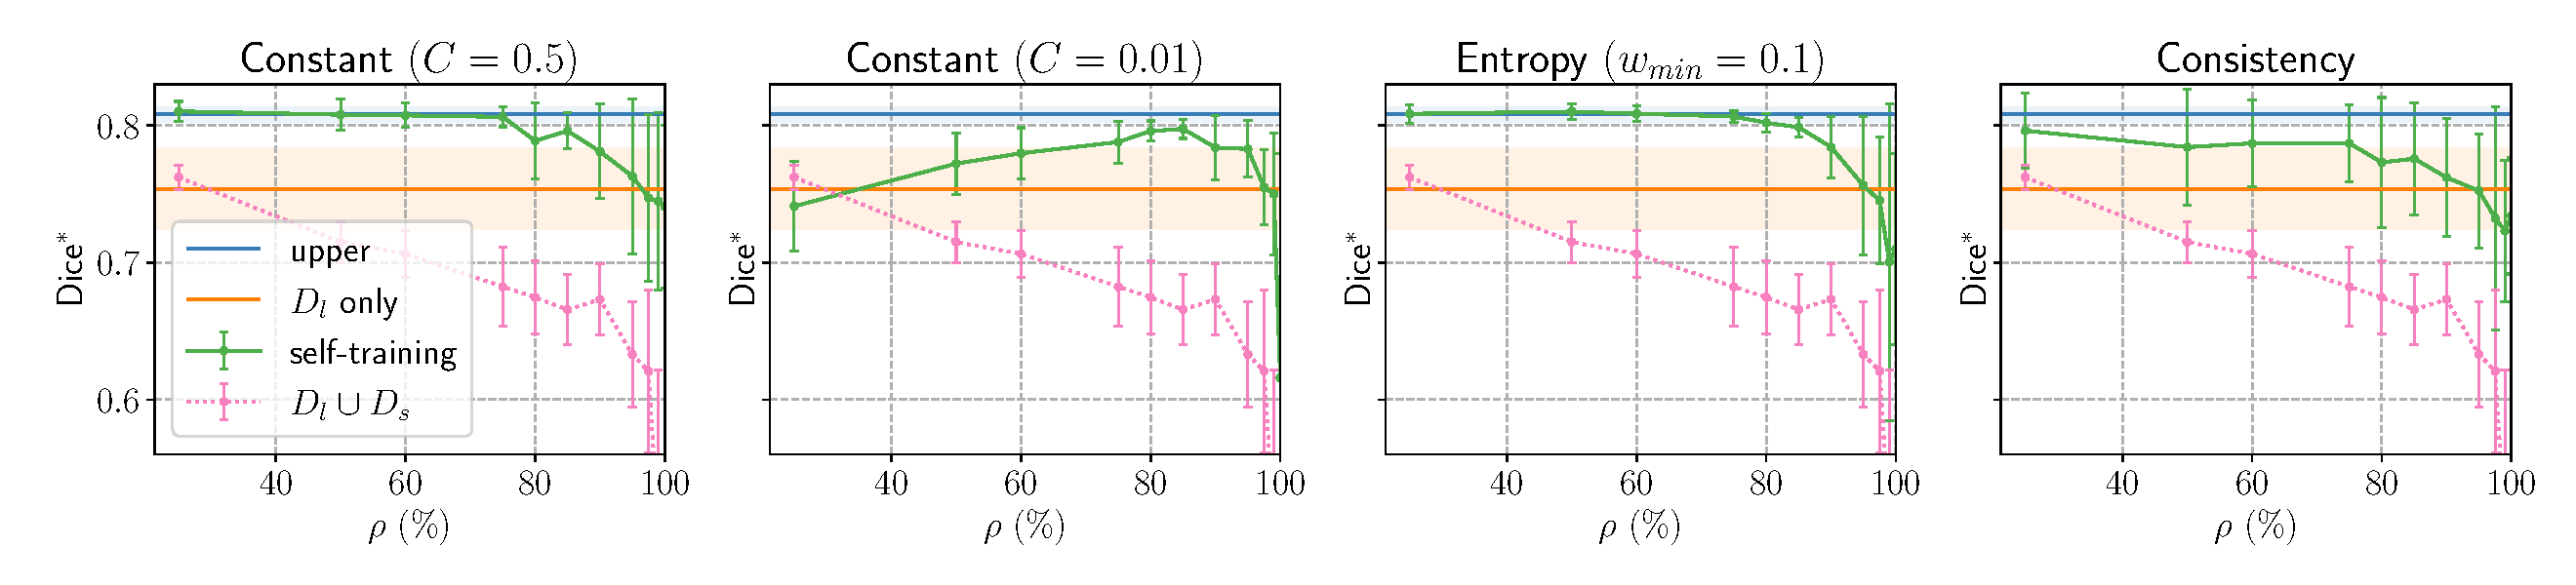
\includegraphics[width=\textwidth]{strain/monuseg_test_pxl_self_hard_dice_rho.pdf}
    \caption{\acrshort{monuseg}}
      \label{fig:strain:rho_exp_monuseg}
  \end{subfigure} \\
  \begin{subfigure}{\textwidth}
    \centering
    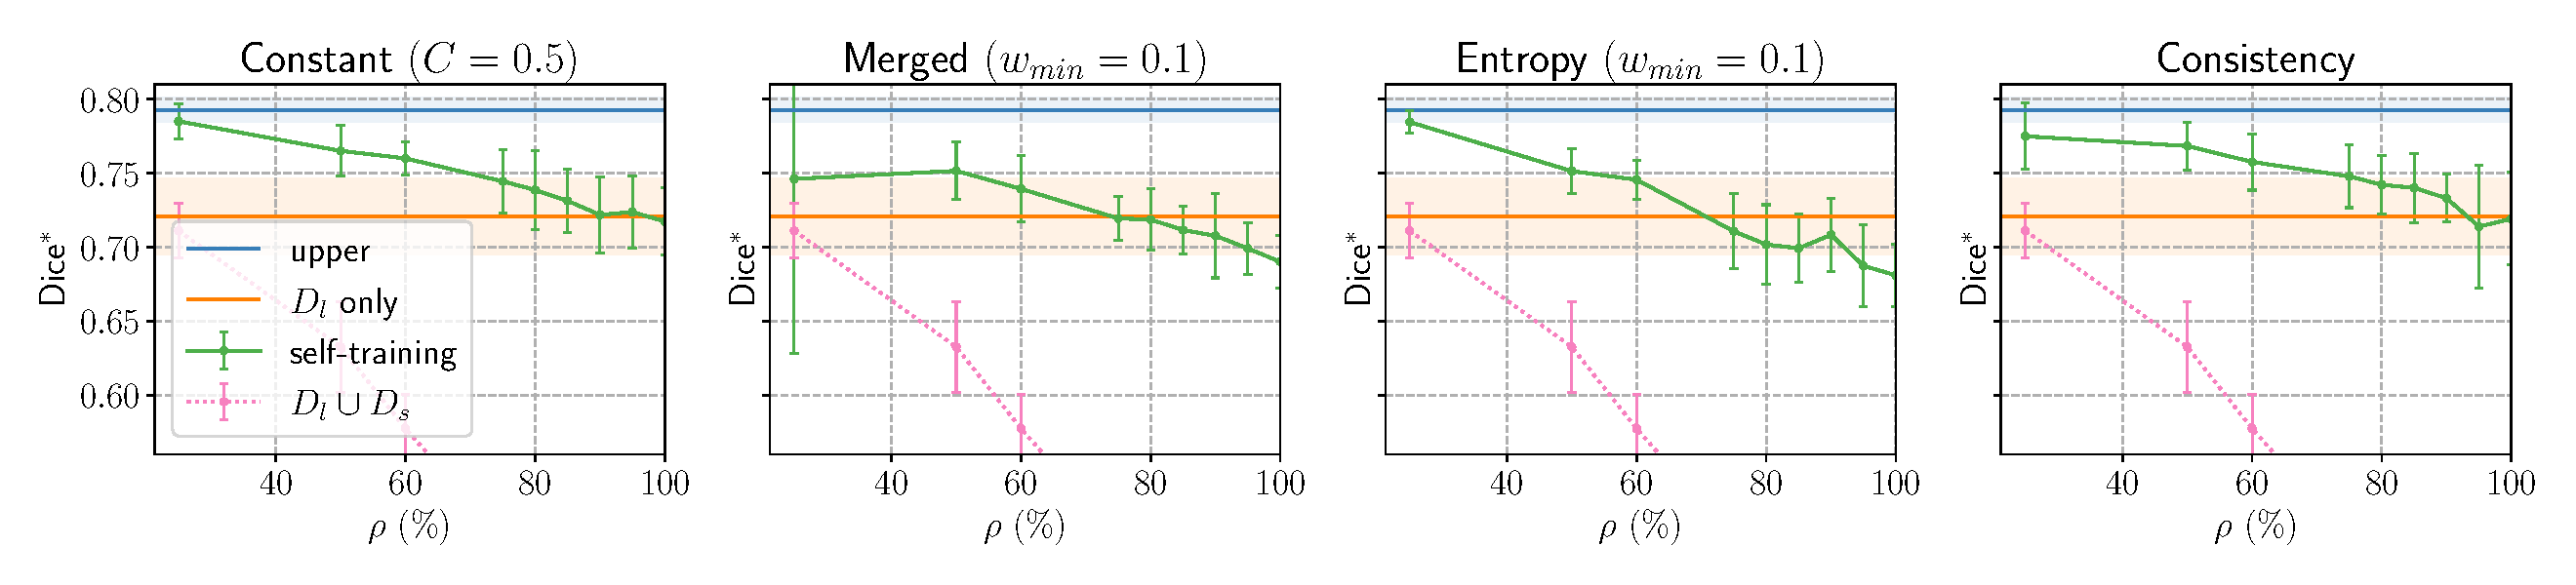
\includegraphics[width=\textwidth]{strain/segpc_test_pxl_self_hard_dice_rho.pdf}
    \caption{\acrshort{segpc}}
    \label{fig:strain:rho_exp_segpc}
  \end{subfigure} \\
  \begin{subfigure}{\textwidth}
    \centering
    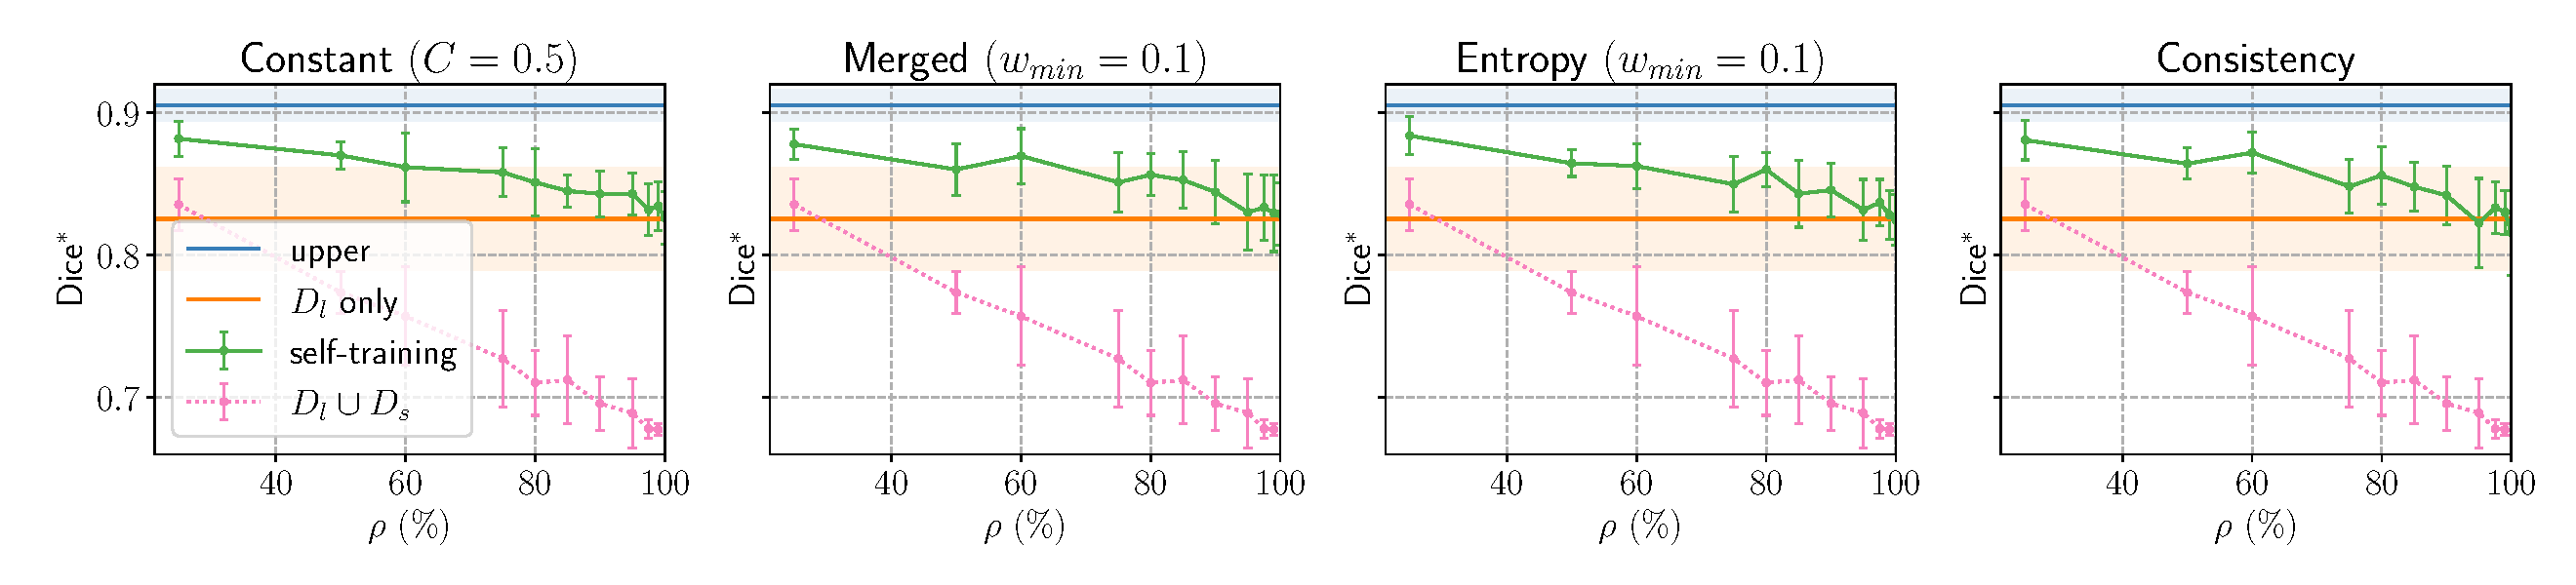
\includegraphics[width=\textwidth]{strain/glas_test_pxl_self_hard_dice_rho.pdf}
    \caption{\acrshort{glas}}
    \label{fig:strain:rho_exp_glas}
  \end{subfigure}
  \caption{Performance of our baselines and self-training approaches with different hyperparameters combinations with a varying $\rho$ and a fixed labeled set size $n_l$. We only report the weighting schemes that show representative behavior. Other weighting strategies are evaluated and reported in Supplementary Section \ref{app:strain:sec:additionalfixednl}.}
  \label{fig:strain:rho_exp}
\end{figure}

\paragraph{\acrshort{monuseg}.} On this dataset, we can divide the analysis by differentiating three scarcity regimes: extreme ($\rho \in [95\%, 100\%]$), significant ($\rho \in [80\%, 90\%]$) and medium ($\rho \in [25\%, 75\%]$). Overall, most self-training approaches benefit from additional sparse annotations as their score increase when $\rho$ decreases. This statement is true for all weighting strategies but the ``\textit{constant}'' with $C = 0.1$ of which the performance plateau near $\rho = 85\%$, before decreasing as $\rho$ decreases. 

In the extreme regime, all self-training approaches exhibit high variance and are outperformed by the ``\textit{$\mathcal{D}_l$ only}'' baseline, or yield comparable performance. In this situation, it appears to be better to work in a fully supervised fashion using only images from $\mathcal{D}_l$ rather then using our self-training approach. Indeed, it seems that the noise brought by the extreme annotation sparsity (or complete lack of annotation when $\rho = 100\%$) degrades the model significantly which cannot even make efficient use of the exhaustively labeled images anymore. For $\rho = 95\%$, two self-training approaches (``\textit{constant}'' with $C = 0.1$ and ``\textit{entropy}'') are on average better then the baseline but variance is still high making it difficult to really conclude that they are more efficient. 

The situation is reversed in the significant regime where most self-training approaches (except the ``\textit{consistency}'' weighting strategy) outperform the ``\textit{$\mathcal{D}_l$ only}'' baseline and variance decreases significantly as well. As for the ``\textit{upper}'' baseline, it remains more efficient than self-training. For $\rho = 90\%$, the most efficient weighting strategy on average is ``\textit{constant}'' with $C = 0.1$ which also exhibits the smallest variance of all the self-training approaches. We believe that such a low constant is particularly helpful to combat the noise brought by the high sparsity as pseudo-labeled pixels contribute way less during training. For $\rho = 85\%$ and $90\%$, the ``\textit{constant}'' with $C = 0.1$ strategy plateaus whereas others catch up in terms of performance and variance decrease with the ``\textit{entropy}'' and ``\textit{merged}'' (plot for this strategy can be found in Supplementary Figure \ref{app:strain:fig:rho_exp_monuseg}) approaches taking up the lead.

In the medium regime, three self-training approaches reach, and even slightly surpass, the upper baseline: ``\textit{constant}'' with $C = 0.5$, ``\textit{entropy}'' and ``\textit{merged}''. This result is interesting because it means that our self-training approach is able to reach the performance of a fully supervised approach but using only $\sim 30\%$ of the original annotations (\ie $\rho = 75\%$, approximately 5k annotations instead of 17k) which is a significant annotation budget saving. The approach ``\textit{constant} $(C=0.1)$'' decreases with $\rho$ indicating that such a low $C$ prevents the model to learn efficiently from the additional annotations (compared to the significant regime). This strategy even finished below the $\mathcal{D}_l \cup \mathcal{D}_s$ baseline at $\rho = 25\%$. 

Overall, results on \acrshort{monuseg}  are quite satisfactory. Although our approach is struggling in an extreme scarcity regime, it quickly catches up with the ``\textit{upper}'' baseline as one adds more annotations to $\mathcal{D}_s$. In this case, the choice of weighting strategy matters and depends on the sparsity of the dataset.

\paragraph{\acrshort{segpc}.} Regarding the trend, our self-training approach behaves similarly on \acrshort{segpc} (see Figure \ref{fig:strain:rho_exp_segpc}) compared to \acrshort{monuseg}: all self-training approaches without exception seem to benefit from additional annotations in $\mathcal{D}_s$. Moreover, the $\mathcal{D}_l \cup \mathcal{D}_s$ baseline is particularly inefficient and finishes just below the ``\textit{$\mathcal{D}_l$ only}'' baseline at $\rho = 25\%$. However, in the extreme regime, the gap between self-training and the ``\textit{$\mathcal{D}_l$ only}'' baseline is less than on \acrshort{monuseg}. The rate at which our approach improves over the ``\textit{$\mathcal{D}_l$ only}'' is also slower as it takes a larger $\rho$ (around $75\%$) for the performance of self-training to become significantly better than this baseline. The best-performing weighting strategies also differ. The best strategies overall are ``\textit{constant}'' (with $C = 0.5$ or $1$) and ``\textit{consistency}''. The ``\textit{merged}'' and ``\textit{entropy}'' are worse than the others, although the latter catches up at $\rho = 25\%$. On this dataset, only the ``constant`` and ``entropy'' strategies come close to catching up with the upper baseline but it takes proportionally more annotations compared to \acrshort{monuseg} as it happens around $\rho = 25\%$.

\paragraph{\acrshort{glas}.} On this dataset, all self-training approaches benefit from additional sparse annotations in $\mathcal{D}_s$. Compared to the ``\textit{$\mathcal{D}_l$ only}'' baseline, the self-training approaches are never worse, even in the extreme scarcity regime, and it takes a $\rho$ between $60\%$ and $75\%$ for self-training to become significantly better. Self-training is not able to catch up the ``\textit{upper}'' baseline in this case. 

\subsection{Labeling a new dataset: sparsely or exhaustively?}
\label{ssec:strain:sparsevsexhaustive}

The fact that self-training is able to equal or outperform the ``\textit{$\mathcal{D}_l$ only}'' and ``\textit{upper}'' baselines suggests that it might be more interesting to consider an alternative annotation strategy to exhaustive labeling when annotating a new dataset. %Therefore, we have conducted an experiment where we % investigate whether or not 
It might indeed be more interesting to combine sparse labeling and self-training rather than performing fully supervised training on an exhaustively labeled dataset (\ie $\mathcal{D}_l$ only). To answer this question, we have conducted a set of experiments where we compare a self-training approach (entropy weighting strategy, $w_{min} = 0.1$) and the baselines all run against different sparsity regimes, varying both $\rho \in \{90\%, 50\%, 25\%\}$ and $n_l$ (values are dataset specific). The results of these experiments are given in Figures \ref{fig:strain:annot_strat_monuseg}, \ref{fig:strain:annot_strat_segpc} and \ref{fig:strain:annot_strat_glas} where the different values of $n_l$ we have used are also specified. In these plots, the performance of all methods are reported over a common metric, the percentage of annotations used, which can be equated with the annotation budget for creating the dataset.

Our experiments show very dataset-dependent results. On \acrshort{monuseg}, we observe that self-training outperforms supervised training for all tested budgets. This indicates that it would have been more interesting to sparsely annotate this dataset. However, this conclusion does not hold for the other datasets as, within the same annotation budget, using ``\textit{$\mathcal{D}_l$ only}'' outperforms self-training.

This experiment also allows to compare which labeling scheme is better for self-training: for a given annotation budget, is it better to favor a larger set $\mathcal{D}_l$ or to add more sparse annotations in $\mathcal{D}_s$? For \acrshort{monuseg} and \acrshort{segpc}, it appears that, for a similar annotation budget, self-training performance are comparable whatever the values of $n_l$ and $\rho$. Therefore, for those datasets, it does not really matter if the annotation budget is spent for exhaustive or sparse labeling. For \acrshort{glas}, however, there is a performance loss when switching from a lower $\rho$ value to a higher (\eg going from $(\rho, n_l) = (90\%, 40)$ to $(50\%, 8)$ in Figure \ref{fig:strain:annot_strat_glas}). It indicates that, it is more interesting to label images exhaustively rather than sparsely for this dataset.

\begin{figure}[t]
  \centering
  \begin{subfigure}{0.48\textwidth}
    \centering
    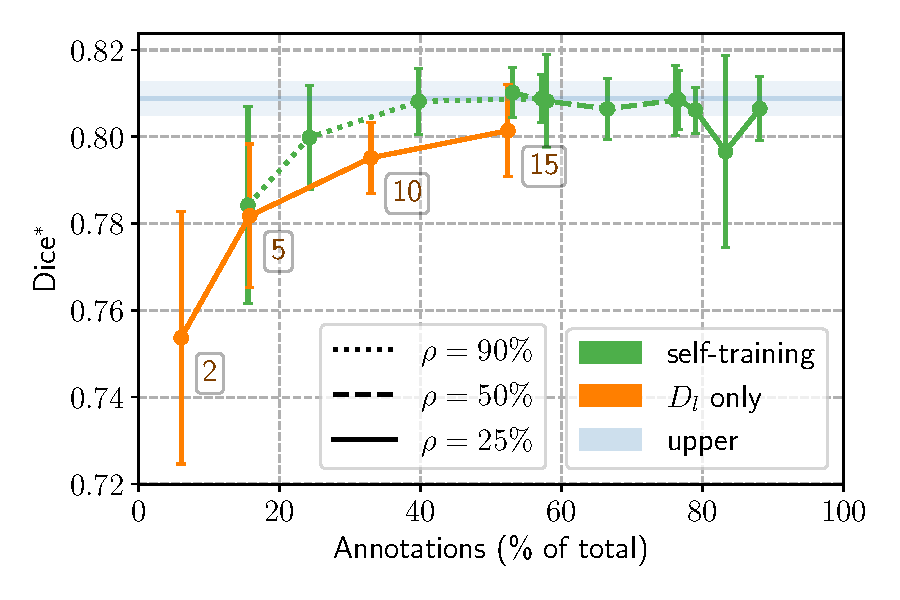
\includegraphics[width=\textwidth]{strain/annot_strat_monuseg.pdf}
    \caption{\acrshort{monuseg}, $n_l = \{2, 5, 10, 15\}$ }
    \label{fig:strain:annot_strat_monuseg}
  \end{subfigure}
  \begin{subfigure}{0.48\textwidth}
    \centering
    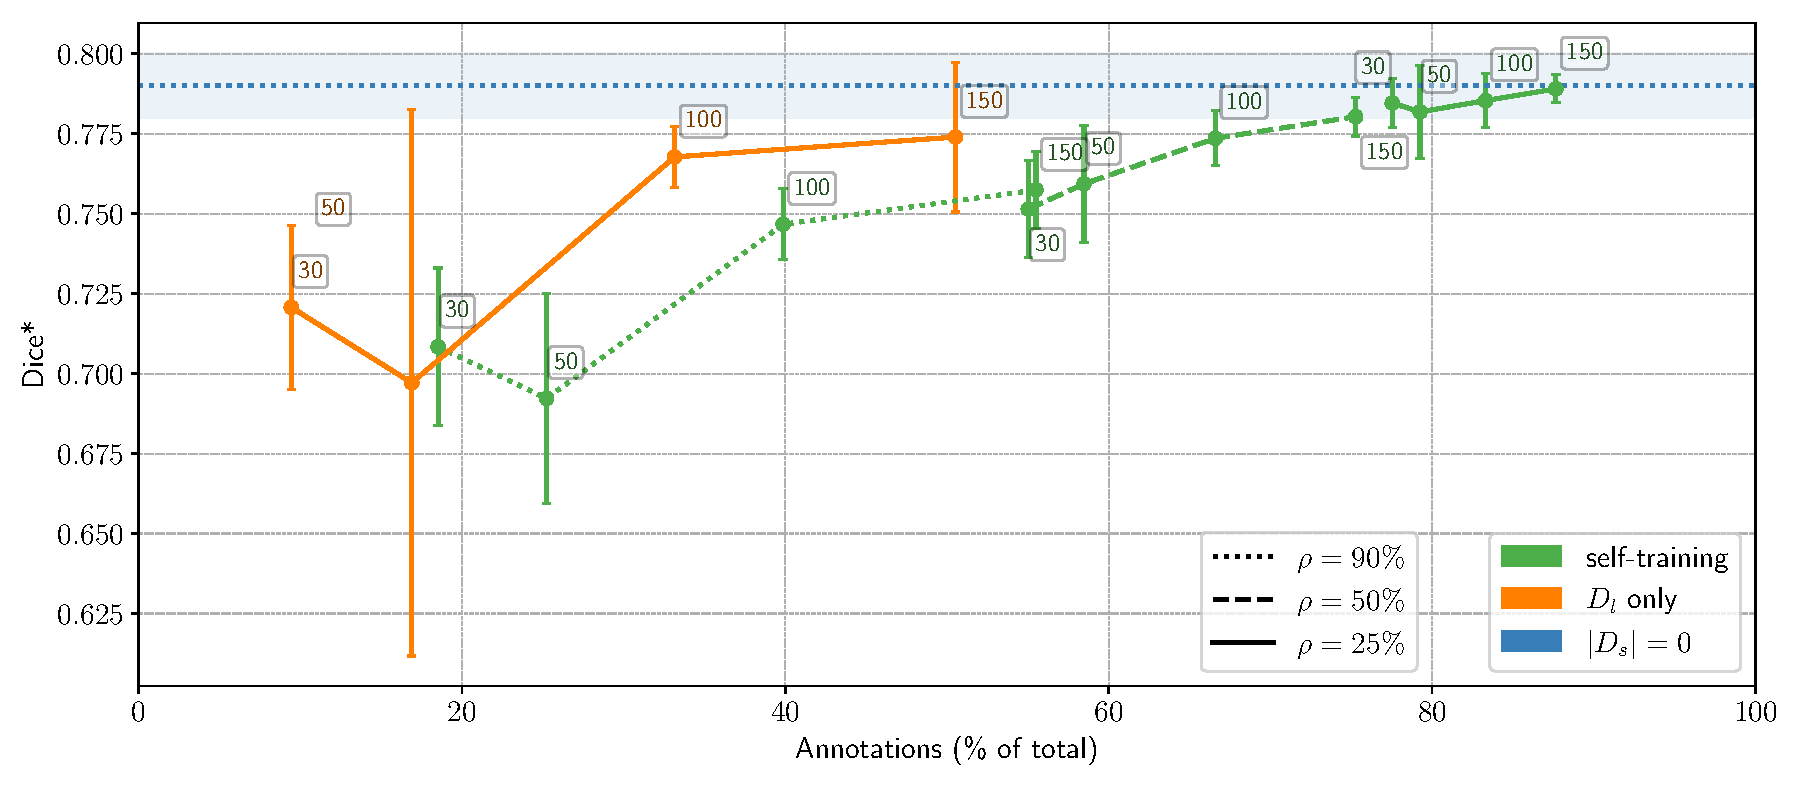
\includegraphics[width=\textwidth]{strain/annot_strat_segpc.pdf}
    \caption{\acrshort{segpc}, $n_l = \{30, 50, 100, 150\}$ }
    \label{fig:strain:annot_strat_segpc}
  \end{subfigure} \\
  \begin{subfigure}{0.48\textwidth}
    \centering
    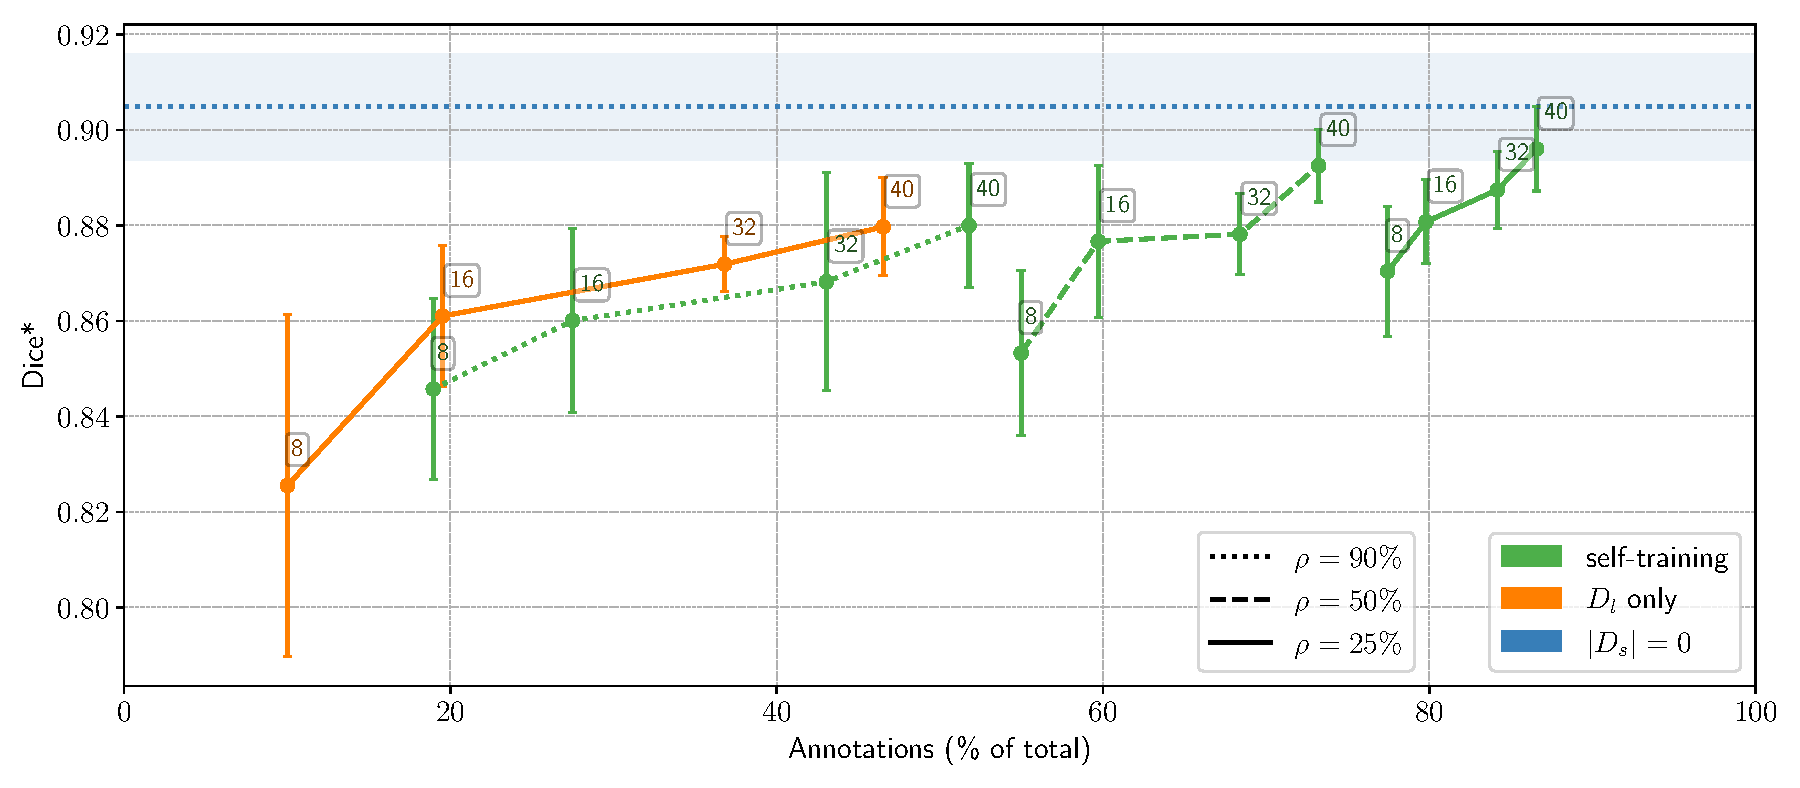
\includegraphics[width=\textwidth]{strain/annot_strat_glas.pdf}
    \caption{\acrshort{glas}, $n_l = \{8, 16, 32, 40\}$ }
    \label{fig:strain:annot_strat_glas}
  \end{subfigure}
  \caption{Performance of self-training \vs the baselines for varying $\rho$ and $n_l$. A point corresponds to 10 runs of a given approach (see line color) and some sparsity parameters, $\rho$ (see line style) and $n_l$ (see subcaptions, increasing from left to right on a constant $\rho$ curve, see ``\textit{$\mathcal{D}_l$ only}'' for example). A new dataset is generated for each run, with the corresponding $n_l$ and $\rho$ values. The $x$ value of a point corresponds to the average percentage of annotations used by the 10 datasets, or, alternatively, to the annotation budget dedicated for labeling the dataset.}
  \label{fig:straing:annot_strat}
\end{figure}

\subsection{Manual threshold tuning}

We have applied ``manual'' threshold tuning to the models produced by the experiments in Section \ref{ssec:strain:fixednl} by re-evaluating them following the procedure described in Section \ref{ssec:strain:evaluation}. In order to study the effects of manual tuning on overfitting, we compare the performance between the performance of tuning the threshold $T$ on $\mathcal{D}_l$, with two test images and one the whole test set. Representative plots for each dataset can be found in Figure \ref{fig:strain:manualtuning}.

As expected, we observe that tuning the threshold $T$ on the training set ($\mathcal{D}_l$) results in overfitting (\ie compared to tuning on $\mathcal{D}_{test}$). However, for two of our three datasets (\acrshort{monuseg} and \acrshort{segpc}), we observe that tuning $T$ on only two test images results in a major performance improvement on average. On \acrshort{glas} however, it seems that using only two images hurts the performance and that, on average, this randomly selected set is overfitted. 

\begin{figure}
  \centering
  \begin{subfigure}{0.48\textwidth}
    \centering
    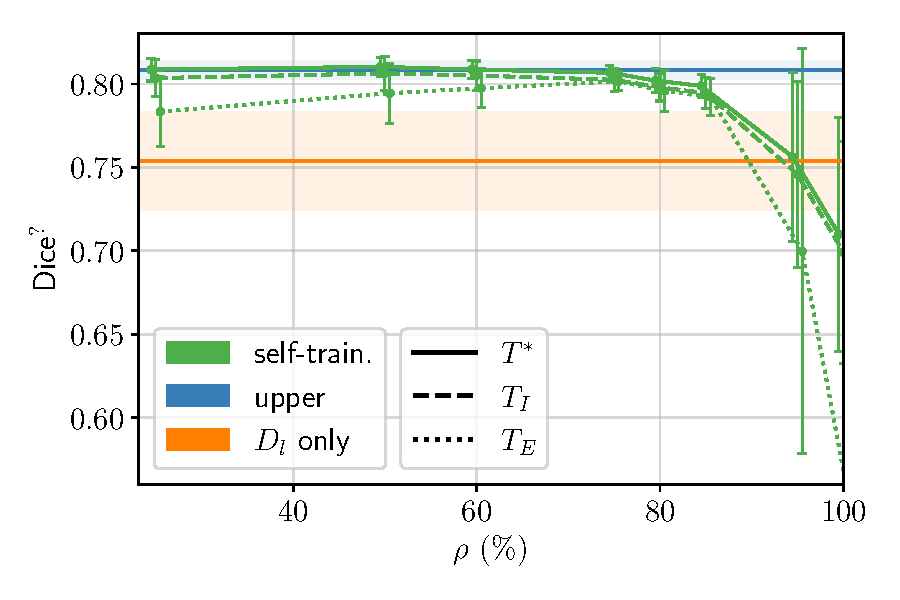
\includegraphics[width=\textwidth]{strain/manualtuning_monuseg_pred_entropy_none.pdf}
    \caption{\acrshort{monuseg}, entropy}
    \label{sfig:strain:manual:monu_entropy}
  \end{subfigure}
  \begin{subfigure}{0.48\textwidth}
    \centering
    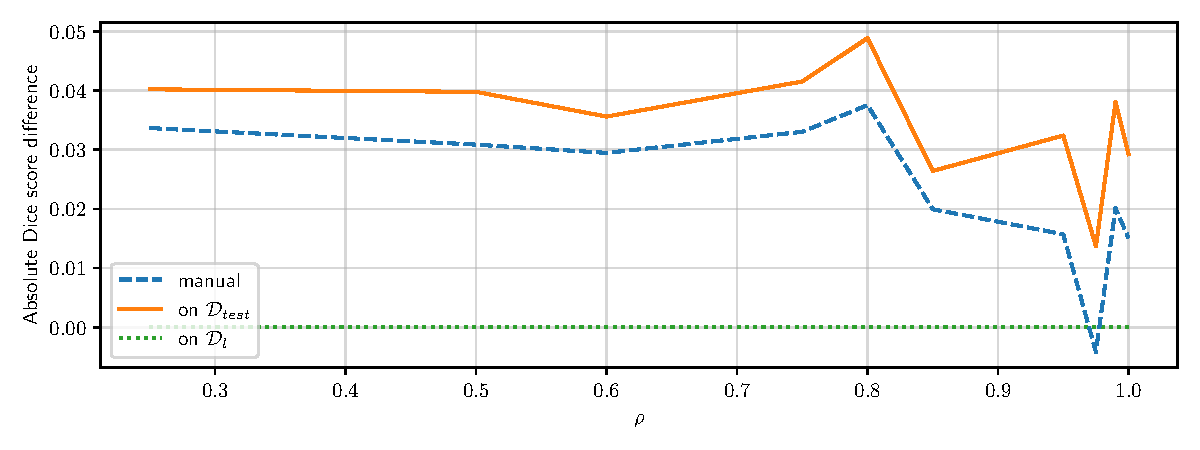
\includegraphics[width=\textwidth]{strain/manualtuning_monuseg_constant_1.0.pdf}
    \caption{\acrshort{monuseg}, constant ($C=1.0$)}
    \label{sfig:strain:manual:monu_constant}
  \end{subfigure} \\
  \begin{subfigure}{0.48\textwidth}
    \centering
    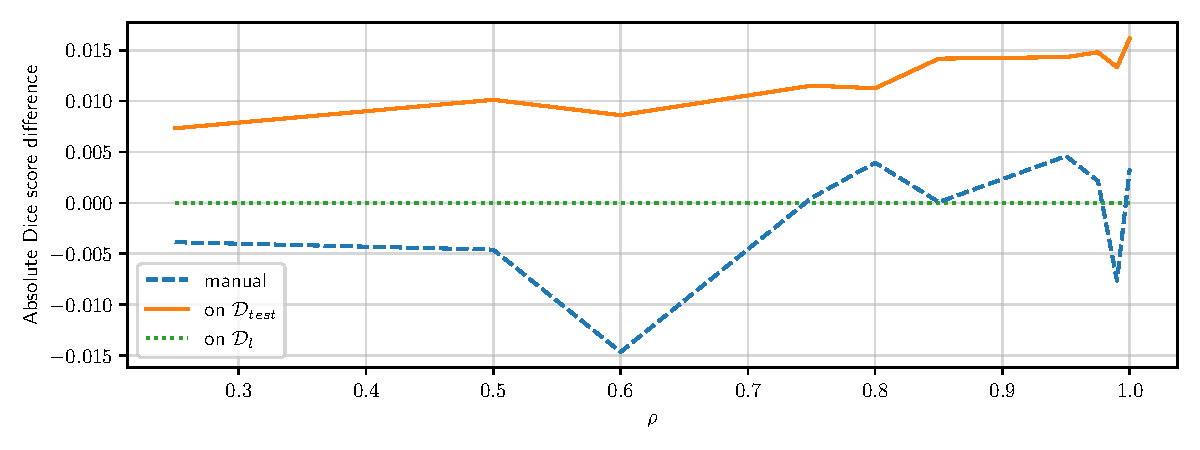
\includegraphics[width=\textwidth]{strain/manualtuning_glas_pred_entropy_none.pdf}
    \caption{\acrshort{glas}, entropy}
    \label{sfig:strain:manual:_glas_pred_entropy_none}
  \end{subfigure}
  \begin{subfigure}{0.48\textwidth}
    \centering
    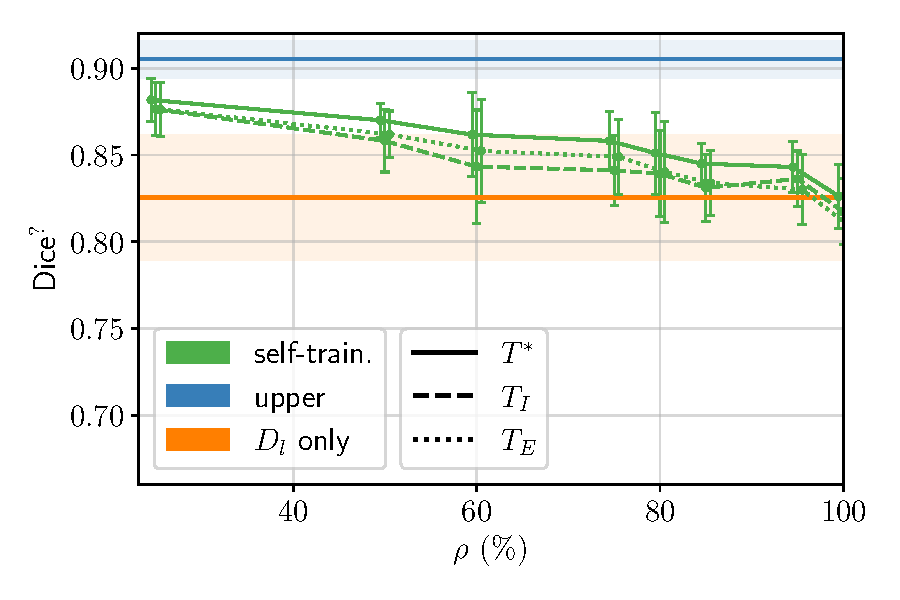
\includegraphics[width=\textwidth]{strain/manualtuning_glas_constant_0.5.pdf}
    \caption{\acrshort{glas}, constant ($C=0.5$)}
    \label{sfig:strain:manual:_glas_constant}
  \end{subfigure} \\
  \begin{subfigure}{0.48\textwidth}
    \centering
    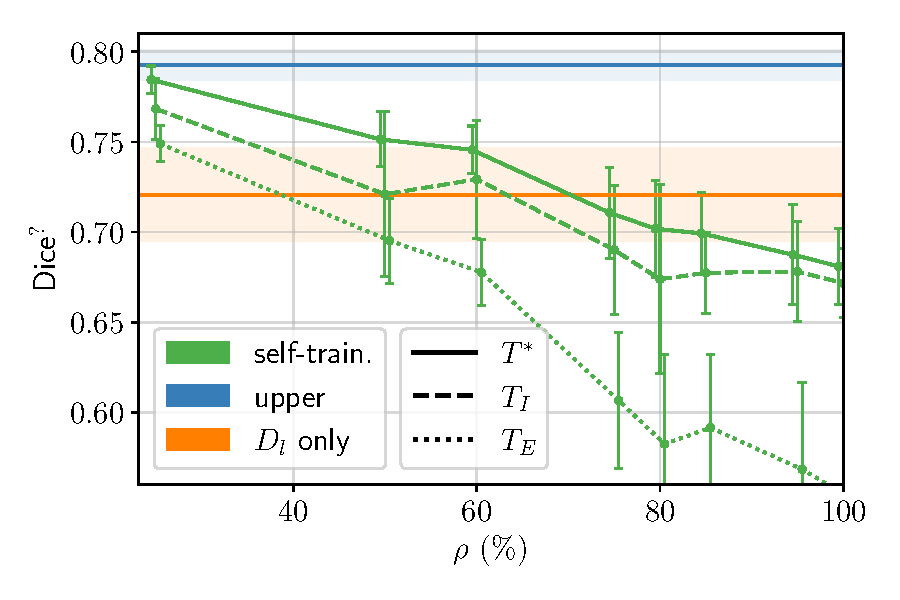
\includegraphics[width=\textwidth]{strain/manualtuning_segpc_pred_entropy_none.pdf}
    \caption{\acrshort{segpc}, entropy}
    \label{sfig:strain:manual:_segpc_pred_entropy_none}
  \end{subfigure}
  \begin{subfigure}{0.48\textwidth}
    \centering
    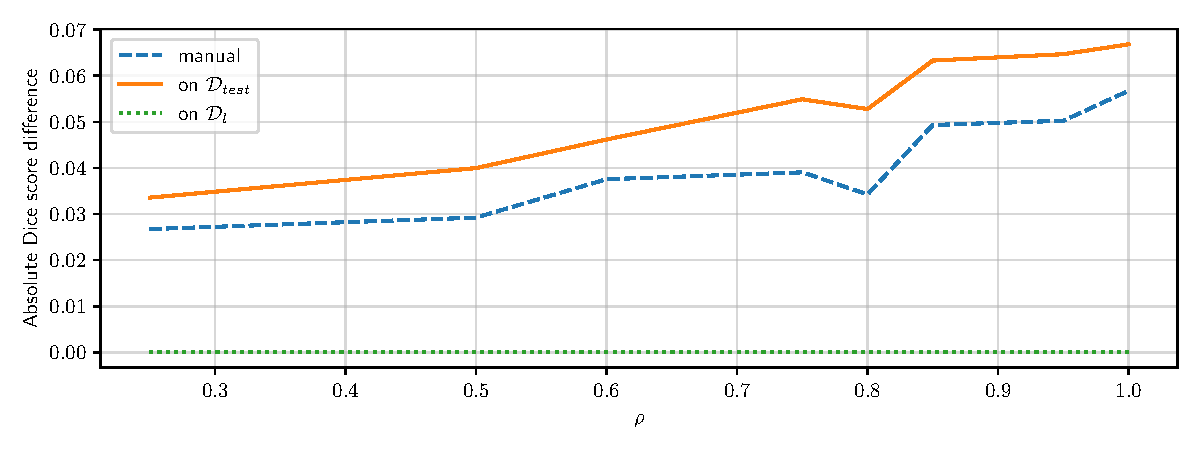
\includegraphics[width=\textwidth]{strain/manualtuning_segpc_constant_0.5.pdf}
    \caption{\acrshort{segpc}, constant ($C=0.5$)}
    \label{sfig:strain:manual:_segpc_constant}
  \end{subfigure}
  \caption{``Manual'' tuning performance. Reported values are the absolute Dice score differences between tuning $T$ on $\mathcal{D}_l$ (dotted green, reference) and approaches where $T$ is tuned on two test images (dashed blue), on the whole test set $\mathcal{D}_{test}$ (solid orange).}
  \label{fig:strain:manualtuning}

\end{figure}


\subsection{Experiments on Thyroid \acrshort{fnab}}
\label{ssec:strain:thyroid_exp}

The Thyroid \acrshort{fnab} dataset introduced in Section \ref{ssec:strain:thyroidfnab} offers a great opportunity to test our method on a real case of sparsely labeled data. It is interesting to note that this dataset is larger than the three public datasets used in this study (almost 5k images in total).

Based on the results of Section \ref{ssec:strain:fixednl}, we have chosen to use the ``\textit{entropy}'' weighting strategy with $w_{min} = 0.1$ for our self-training approach, as it provides consistently good results across datasets. We compare this approach with two of our three baselines: ``\textit{$\mathcal{D}_l$ only}'' and ``$\mathcal{D}_l \cup \mathcal{D}_s$''. The ``\textit{upper}'' baseline obviously cannot be evaluated because we do not have access to the complete ground truth. The resulting performances are given in Table \ref{tab:strain:thyroidresults}.

We observe that our self-training approach significantly outperforms the two baselines and remains quite stable as its standard deviation is below $1\%$. This confirms the interest of self-training when working with a sparse dataset. 

\begin{table}[t]
  \centering 
  \begin{tabular}{|c|c|}
    \hline
    Method & $\text{Dice}^*$ \\
    \hline
    Self-training & $89.05 \pm 0.85$ \\
    $\mathcal{D}_l$ only & $80.30 \pm 5.39$\\  
    $\mathcal{D}_l \cup \mathcal{D}_s$ & $83.62 \pm 3.52$\\
    \hline
  \end{tabular}
  \caption{Experiment on the Thyroid \acrshort{fnab} dataset. The self-training approach uses the ``\textit{entropy}'' weighting strategy and $w_{min} = 0.1$.}
  \label{tab:strain:thyroidresults}
\end{table}

\section{Conclusion}
\label{sec:strain:conclusion}

In this work, we have introduced a method based on self-training for training a deep binary segmentation model with sparsely labeled data. Using 4 datasets, including an actual sparsely labeled one, we have shown that the method could indeed make use of sparse annotations to improve model performance over using only exhaustively labeled data. For one of our datasets, our self-training approach using only $30\%$ of the original training annotations is even able to reach performance comparable to using all of them in a supervised way.

In the future, we want to extend the method to multi-class segmentation and further study the impact of various training choices and hyperparameters (model complexity, weighting strategies, soft pseudo-labeling, \etc.) that we could not explore due to time and computing resources constraints. We also want to further study how the type of dataset (variability in images, density of ground truth, large or small annotations, \etc.) impacts the performance margins of self-training. Moreover, in this work, we have removed annotation randomly from the datasets. In practice, it is unlikely that the existing annotations are really randomly chosen and it would be interesting to study the effect of the labeling process. This work has mostly been focused on high scarcity conditions but self-training methods have also shown to be beneficial with very large labeled and unlabeled sets in other contexts. In computational pathology, whole slide images usually offer a great potential for a large pool of unlabeled data. Therefore, we would like to study how our method would perform in such a context. Finally, we would also like to explore how our self-training algorithm could be used in an interactive mode to assist new dataset labeling. %Eventually, we want to implement the algorithm on the Cytomine platform. 

